\chapter{TileCal PMT response in calibration transfer analysis}
\label{app:pmt}

This appendix describes the impact of a non linearity in the response of the \gls{tilecal} \glspl{pmt} 
on the luminosity calibration transfer analysis; 
this is used to estimate the uncertainty in the luminosity due to the extrapolation between 
low-$\mu$ bunches, where LUCID is calibrated, and the high-$\mu$ bunches of physics runs. 
Correcting for this non-linearity in the \glspl{pmt} allows to considerably reduce the luminosity systematic uncertainty. 

\section{Luminosity calibration transfer}

The general strategy to measure the luminosity in \gls{atlas} is outlined in Section \ref{sec:lumimeas}.
LUCID is the \gls{atlas} detector that, during \gls{vdm} runs, measures the absolute luminosity. 
LUCID algorithms are non-linear with $\mu$, and this non-linearity is corrected with the calibration transfer, 
which  
allows to extrapolate the absolute LUCID calibration from conditions corresponding to few low-$\mu$, isolated bunches 
to the conditions of the physics runs, where there are many high-$\mu$ bunches in trains. 

The default system used to provide the calibration transfer is the tracking system. As already discussed in Section \ref{sec:lumimeas},
the number of reconstructed tracks in the \gls{id} is proportional to $\mu$. 
The track selection that is used for the calibration transfer corresponds to the TightPrimary quality criteria but dropping 
the requirement on the Pixel holes (that have to be $\leq 1$ for the standard TightPrimary selection);
furthermore there is a requirement on the impact parameter significance, $|d_0|/\sigma(d_0)<7$, and on 
the pseudorapidity of the track, $|\eta|<1$. These criteria have been optimized to reduce the dependence on the Pixel conditions. 

The procedure to determine the calibration transfer assumes that the tracking luminosity measurement 
(in the following referred to as "Tracking") 
does not have any dependence on $\mu$ or on the position in the train, and it consists of three steps:
\begin{enumerate}
\item The bunch-averaged track luminosity during the \gls{vdm} run is normalized to the LUCID luminosity (which in these runs 
undergo the absolute calibration). The \gls{vdm} runs have low-$\mu$ isolated bunches.
\item The ratio of the luminosity measured by LUCID and Tracking is measured as a function of $\mu$ (as measured by LUCID) 
in a single run with high-$\mu$ trains. The distribution of the values of this ratio is fitted with a straight line.
\item The result of the fit is used to apply a correction to the luminosity measured by LUCID in physics runs. 
%Fit the relative mu-dependence between the two in a single calibration-transfer run with high-mu trains. In the plot: x-axis mu measured by lucid. y: ratio of Tracking to lucid luminosity. Fit the line. The mu dependence corresponds to an 11\% correction at mu=50 to the lucid response. This is a large number that we have to control at sub-percent level. 
%Apply to LUCID in physics runs 
\end{enumerate}

\begin{figure}[ht]
\centering
\subfigure{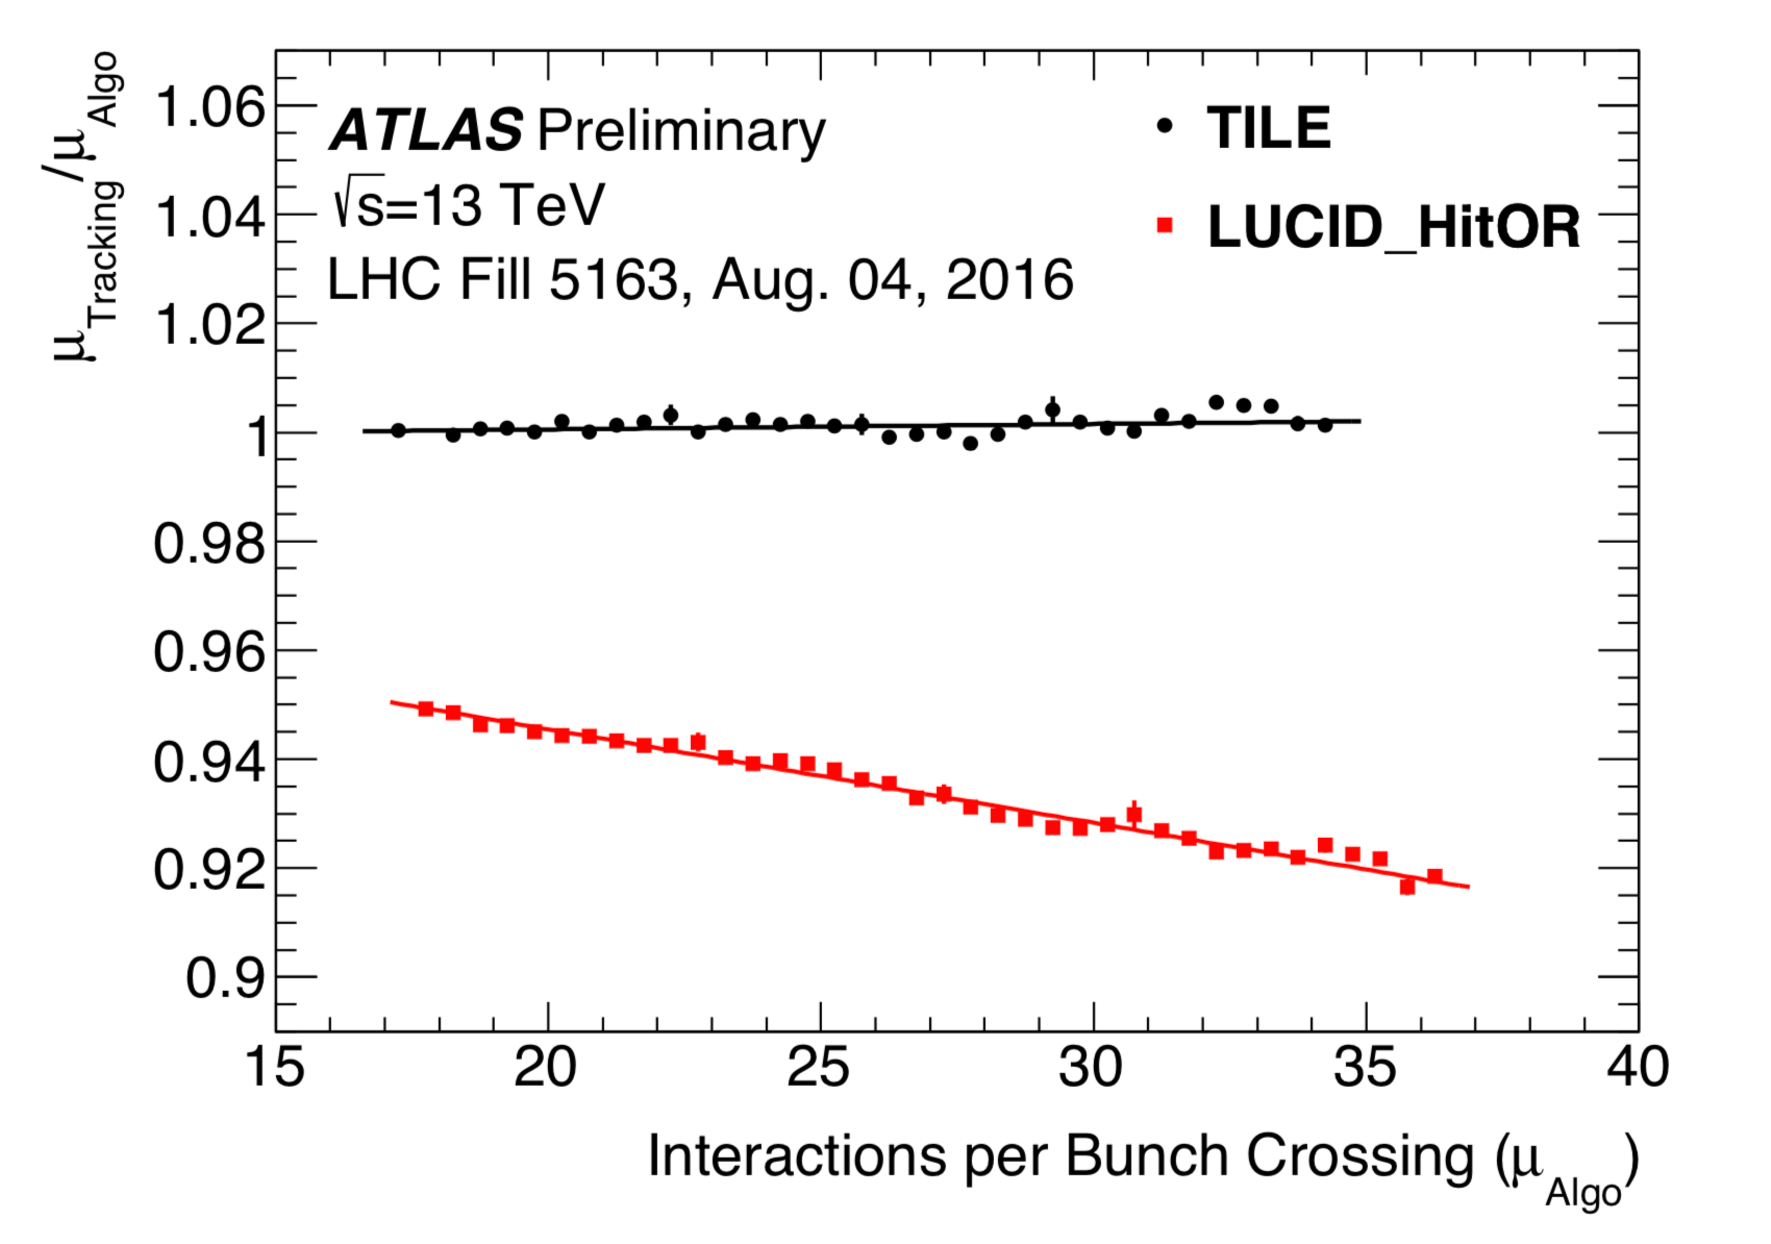
\includegraphics[width=0.65\textwidth]{figures/pmt_response/calibration_transfer_track.pdf}}
\caption{Ratio of the Tracking luminosity to the luminosity measured by LUCID (red) and \gls{tilecal} (black) as a function of $\mu$.}
\label{fig:apppmt:calib_transfer}
\end{figure}

As it can be observed in Figure \ref{fig:apppmt:calib_transfer}, at high-$\mu$ LUCID overestimates the luminosity and 
the correction factor is as big as 11\% for $\mu \approx 50$. 

To assign an uncertainty to the calibration transfer, a 
procedure similar to that used for the Tracking luminosity 
is repeated using the 
integrator system of the \gls{tilecal} detector, and the relative difference between the luminosity measured by the tracking system and 
by \gls{tilecal}  is used as uncertainty. 
Just like in the case of the luminosity measurement from the tracking system, the \gls{tilecal} luminosity measurement 
relies on some assumptions, in particular the perfect linearity of the \gls{pmt} response over a wide range of instantaneous luminosity, 
which spans over three orders of magnitude. 


\section{TileCal laser system}
\label{sec:app:laser}

The \gls{tilecal} laser system \cite{system:2016tae} is designed with the main purpose of calibrating the \glspl{pmt} and readout chain: 
in absence of collisions, a controlled amount of light is sent to each \gls{pmt}'s photocatode, 
and the response is used to derive the laser calibration constant. 
The laser system has been renewed for Run 2 and the new version (LaserII)
has been installed in October 2014 \cite{Scuri:2016ctn-2}. 
During the calibration, which is performed every two or three days in the 
pauses between the \gls{lhc} collisions,
laser pulses with a wavelength of 532 nm are sent to all \gls{pmt} cathodes 
trough 400 100-meters long fibers. 
The laser light is sent also to monitor photodiodes, to remove the dependence on the laser stability. 

Laser pulses are also sent in the abort gaps during physics runs, with a frequency of 
3 Hz. 
This procedure is used to detect "time jumps", changes in the time settings of groups of channels 
that in Run 1 were particularly frequent after a power restart of the low-voltage power
supply.
The response of the \glspl{pmt} to the laser pulses sent in empty bunches in physics runs 
is also used to perform the analysis described in this appendix. 


\section{PMT response to laser pulses in empty bunches}
\label{sec:app:pmtresponse}

One of the possible techniques of to estimate 
the difference between the Tracking and the \gls{tilecal} measurements of the calibration transfer is the following:
\begin{enumerate}
\item The luminosity of all the \gls{tilecal} cells used is individually calibrated to match the Tracking luminosity 
at a specific high-$\mu$ run (anchor run).
\item Interpolating this value with the origin in the current-luminosity plane allows to derive an estimate for the \gls{tilecal} 
luminosity during the \gls{vdm} run.
\item The comparison of this luminosity with the luminosity measured by the tracking system provides the systematic uncertainty in the 
calibration transfer. 
\end{enumerate}
The measurement of the calibration transfer with \gls{tilecal} needs to take into account two effects that complicate the measurement. 
\begin{itemize}
\item Activation decays after high-$\mu$ runs bias the \gls{tilecal} response in low-$\mu$ runs like the \gls{vdm} run.
\item It has been shown that the \gls{pmt} response is not perfectly linear with the luminosity. 
\end{itemize}

This sections focus on the analysis of this second point and on the corrections derived to minimize its effect 
on the \gls{tilecal} calibration transfer analysis; this allows to reduce the calibration transfer uncertainty in the 
2017 luminosity, which is the dominant luminosity uncertainty for the 2016 dataset. 
The cells we consider for this study are all the E-type cells and A13 (see Figure \ref{fig:atlas:tile_cells}).

It has previously been noticed (see e.g. Ref. \cite{giulia:tesi}) that the \gls{tilecal} \glspl{pmt} show a non-linearity in 
the response with the increase in luminosity. 
In this section we study this effect for the cells and run numbers that are of interest for the 
calibration transfer analysis. 
The anchor run used in the calibration transfer analysis is 331085, while the run number of the \gls{vdm} 
run is 330875.

The \gls{tilecal} laser system is primarily used to calibrate the \gls{tilecal} readout. 
The laser system can also be fired in the abort gaps during standard physics runs; in this case 
one laser pulse is sent three times per second.
The \gls{pmt} response is analyzed in the following steps:
\begin{enumerate}
\item The response of the \glspl{pmt} is normalized to the response of the monitor diode D0 to remove fluctuations 
due to laser instabilities.

\item The distribution of the response for each individual \gls{pmt} in groups of 25 \gls{lub} is considered. 
Grouping together several \glspl{lub} is necessary to accumulate enough data points: the frequency of laser pulses is 3 Hz, 
which gives only about 180 data points per minute. The value of 25 has been chosen for consistency with previous studies, 
after checking that the size of the group of \glspl{lub} does not to affect the results 
as long as it is large enough to provide a sufficiently large number of events.

\item The response for each cell family is computed by averaging over all the \glspl{pmt} 
belonging to that family. We keep separate the left and right \glspl{pmt} and the A and C side 
of \gls{tilecal}.

\item The distribution of the response is normalized to the last group of \glspl{lub} that 
does not contain the \gls{lub} where "stable beams" is declared, which is used as reference.

\end{enumerate} 

Figure \ref{fig:apppmt:331085:variation_A13} shows the \gls{pmt} response for the cell family A13 during the anchor run, 
while Figure \ref{fig:apppmt:331085:variation_E1_E2} shows the response for the cells of the families E1 and E2 
and Figure \ref{fig:apppmt:331085:variation_E3_E4} for the families E3 and E4.
While the origin of this discontinuity in the response is still under investigation, it is clear that 
the drastic change in response happens in correspondence of the declaration of stable beam, when the 
luminosity increases, and is therefore referred to as non-linearity of the \glspl{pmt}. 

\begin{figure}[htbp]
\centering
\subfigure{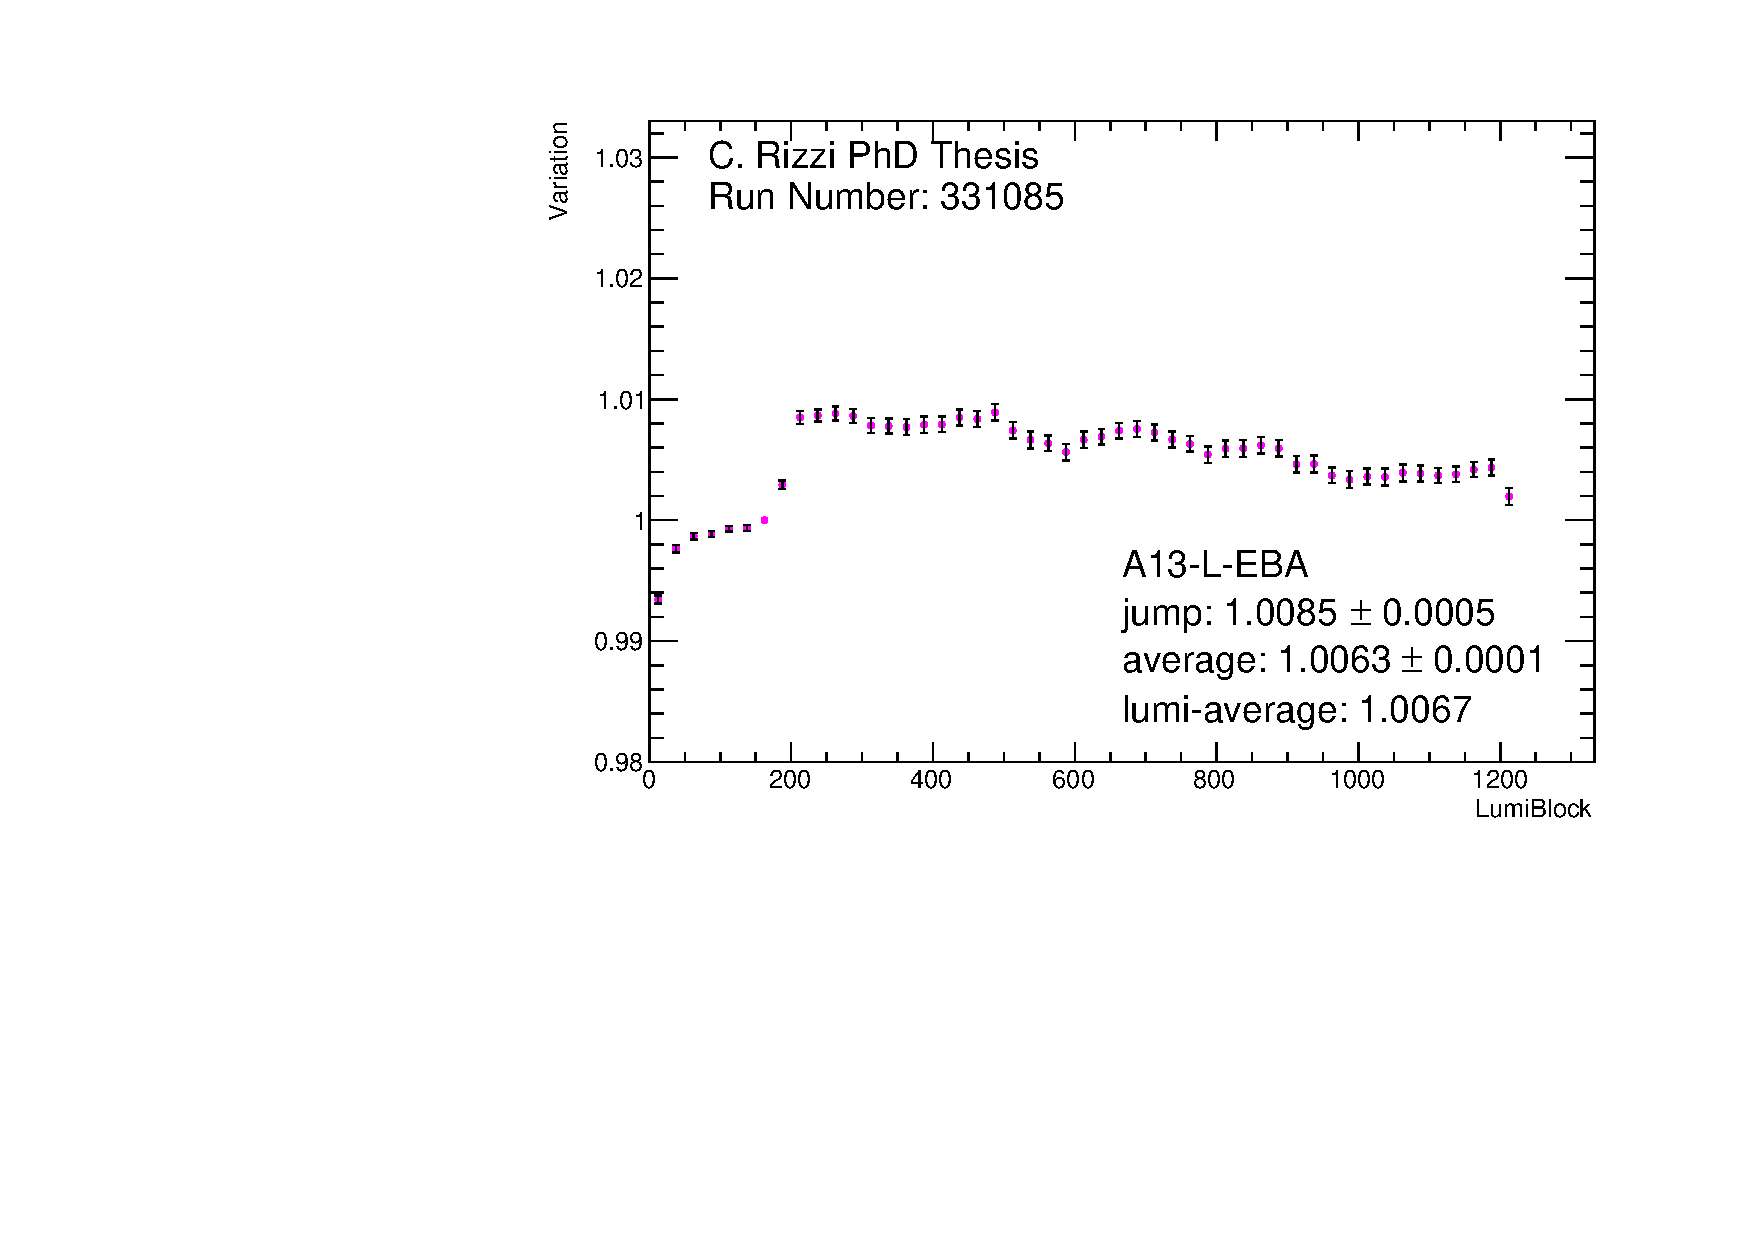
\includegraphics[width=0.45\textwidth]{figures/pmt_response/331085/variation_A13_L_EBA}\label{fig:app:variation_A13_L_EBA}}
\subfigure{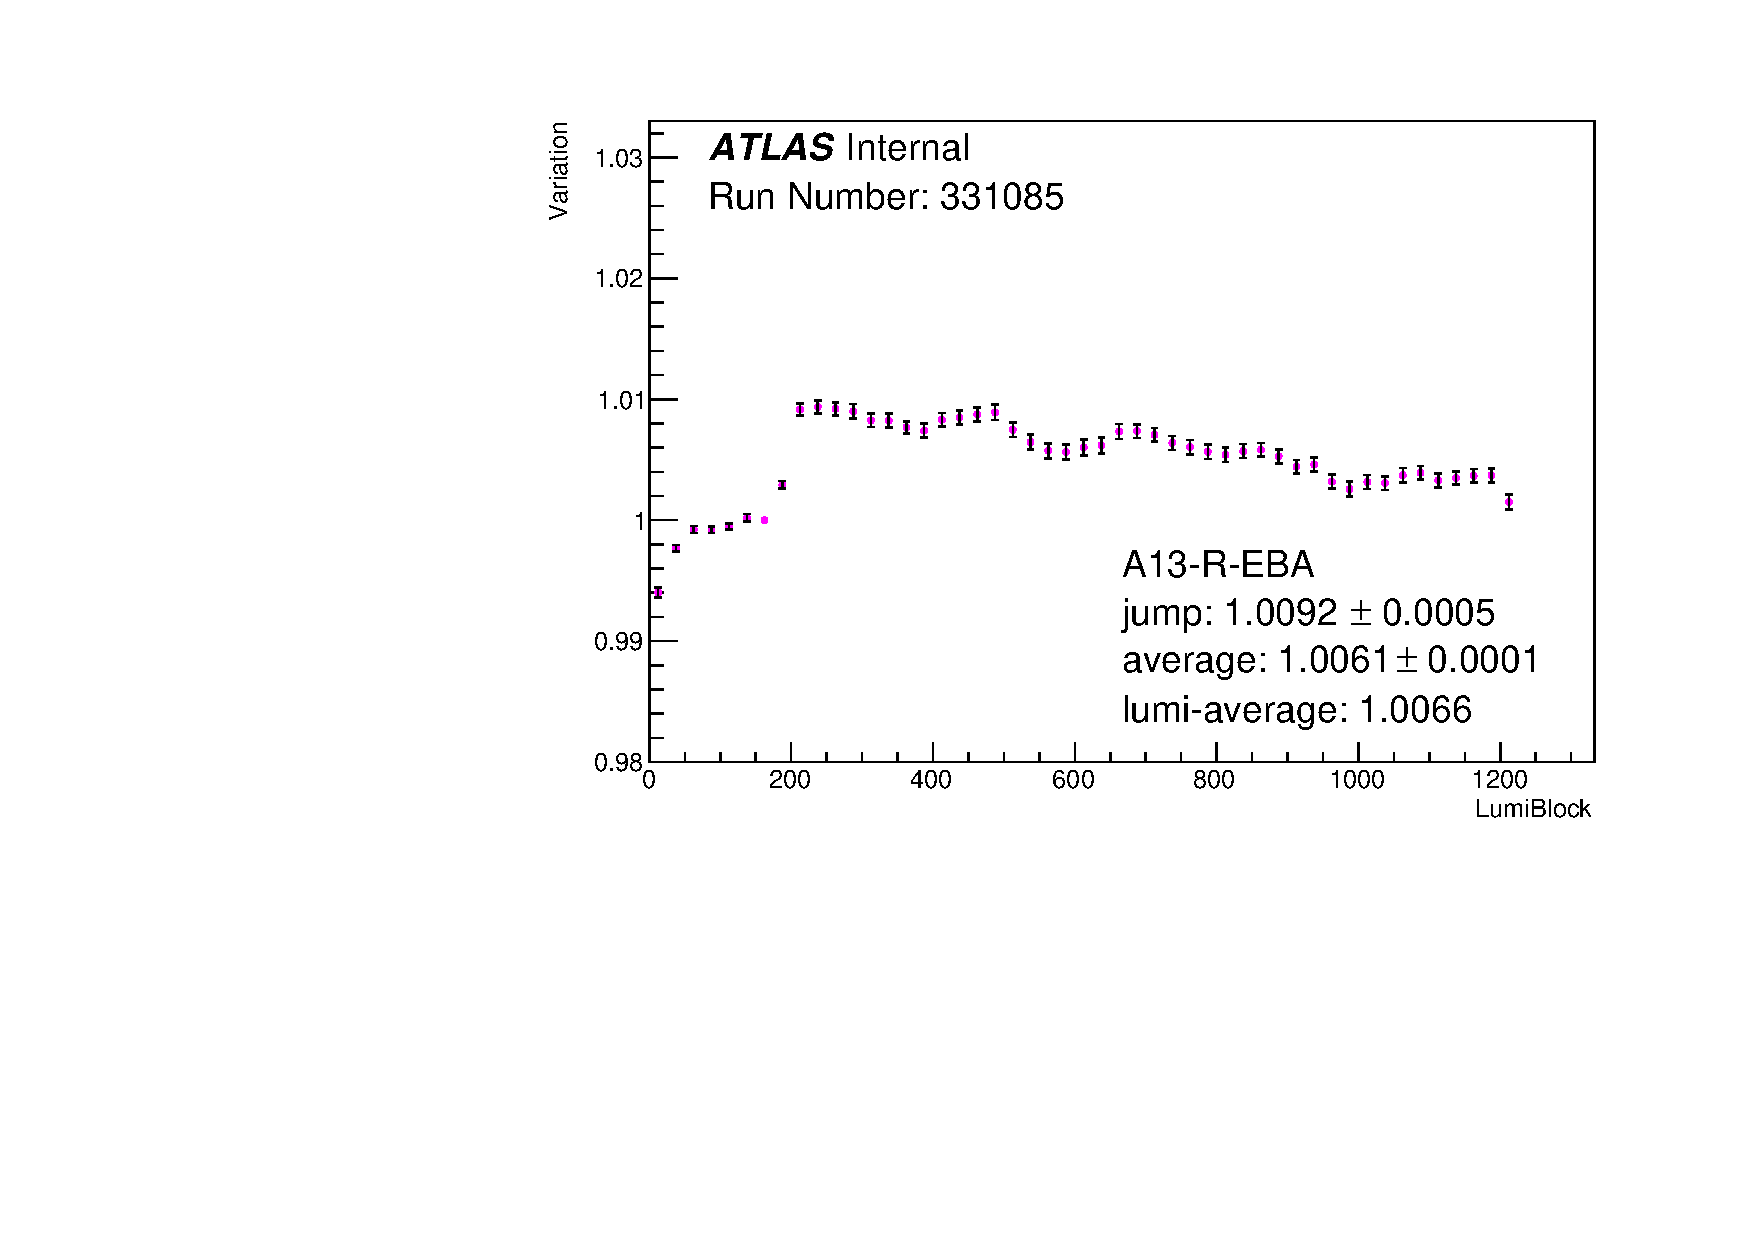
\includegraphics[width=0.45\textwidth]{figures/pmt_response/331085/variation_A13_R_EBA}\label{fig:app:variation_A13_R_EBA}}\\
\subfigure{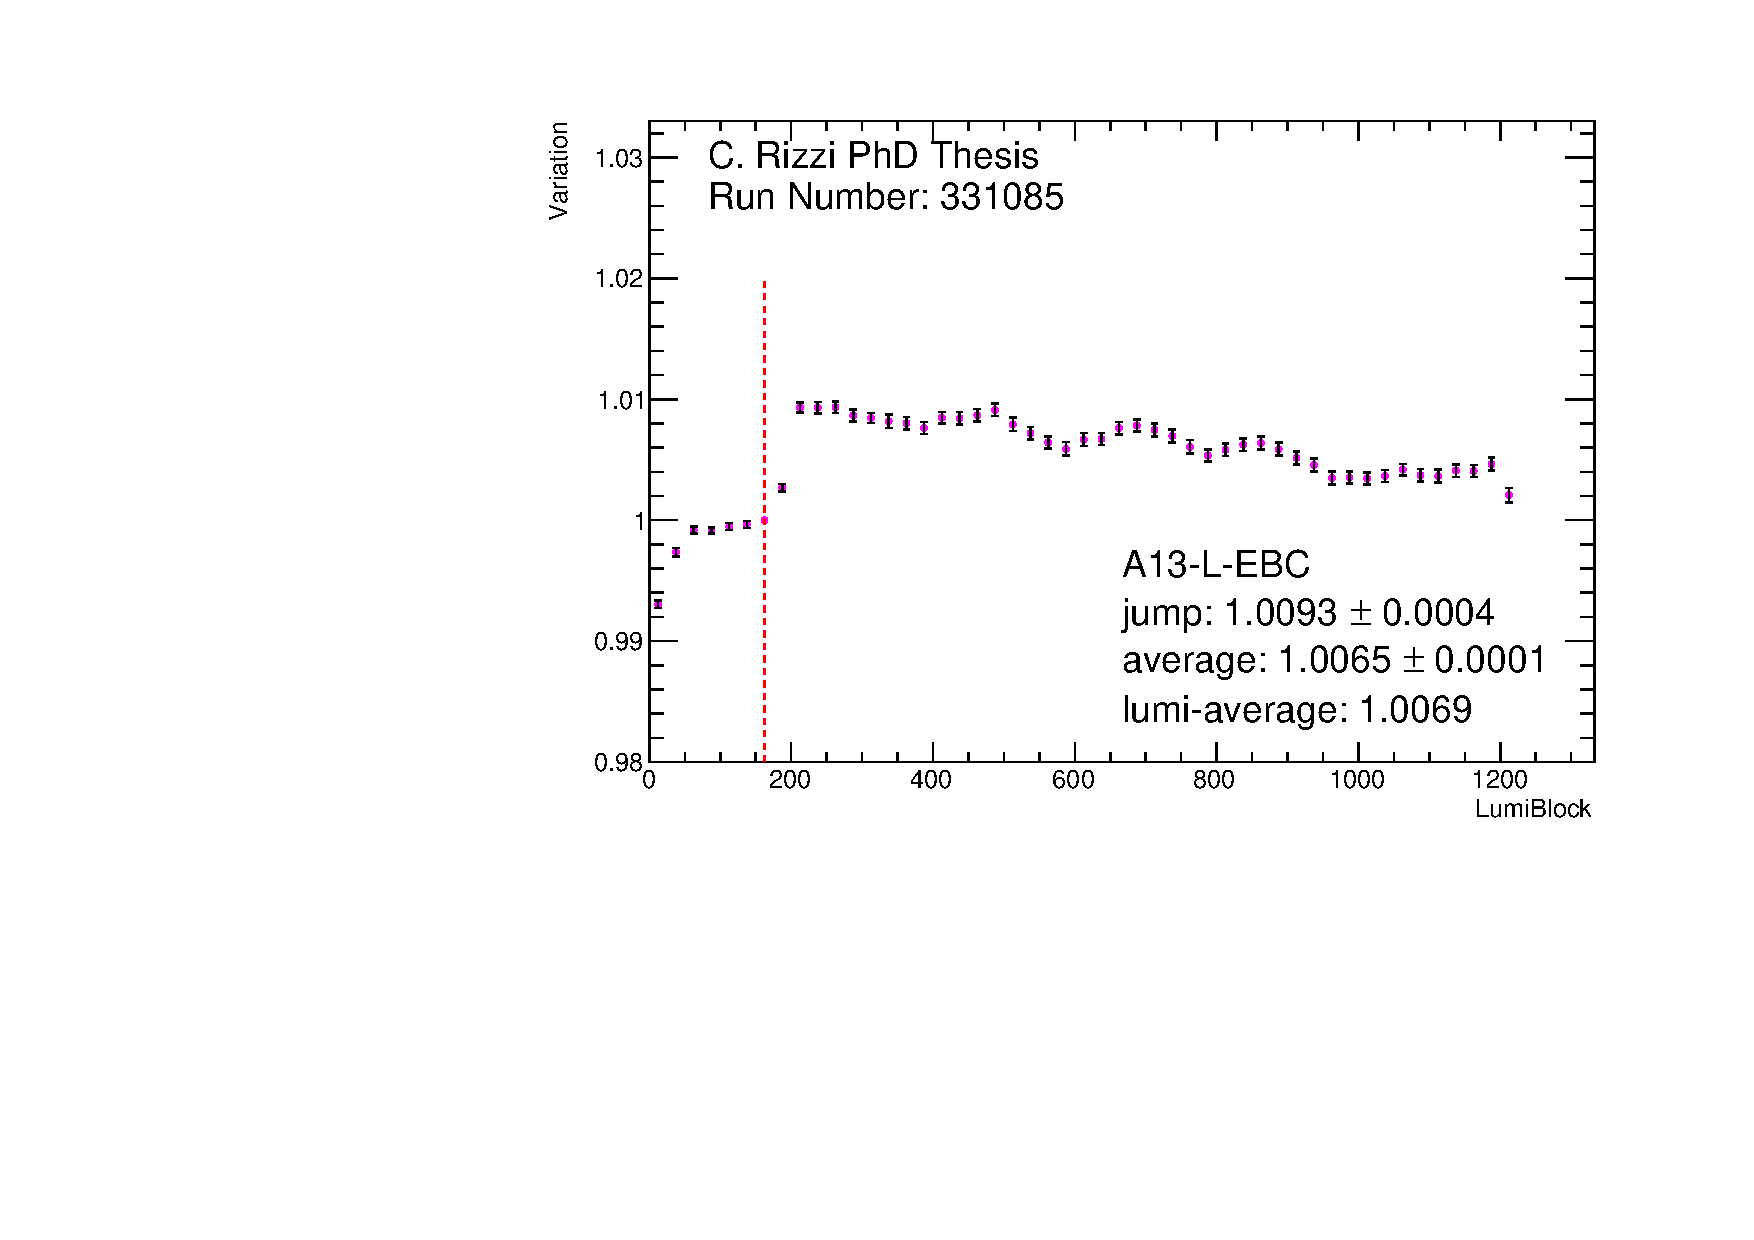
\includegraphics[width=0.45\textwidth]{figures/pmt_response/331085/variation_A13_L_EBC}\label{fig:app:variation_A13_L_EBC}}
\subfigure{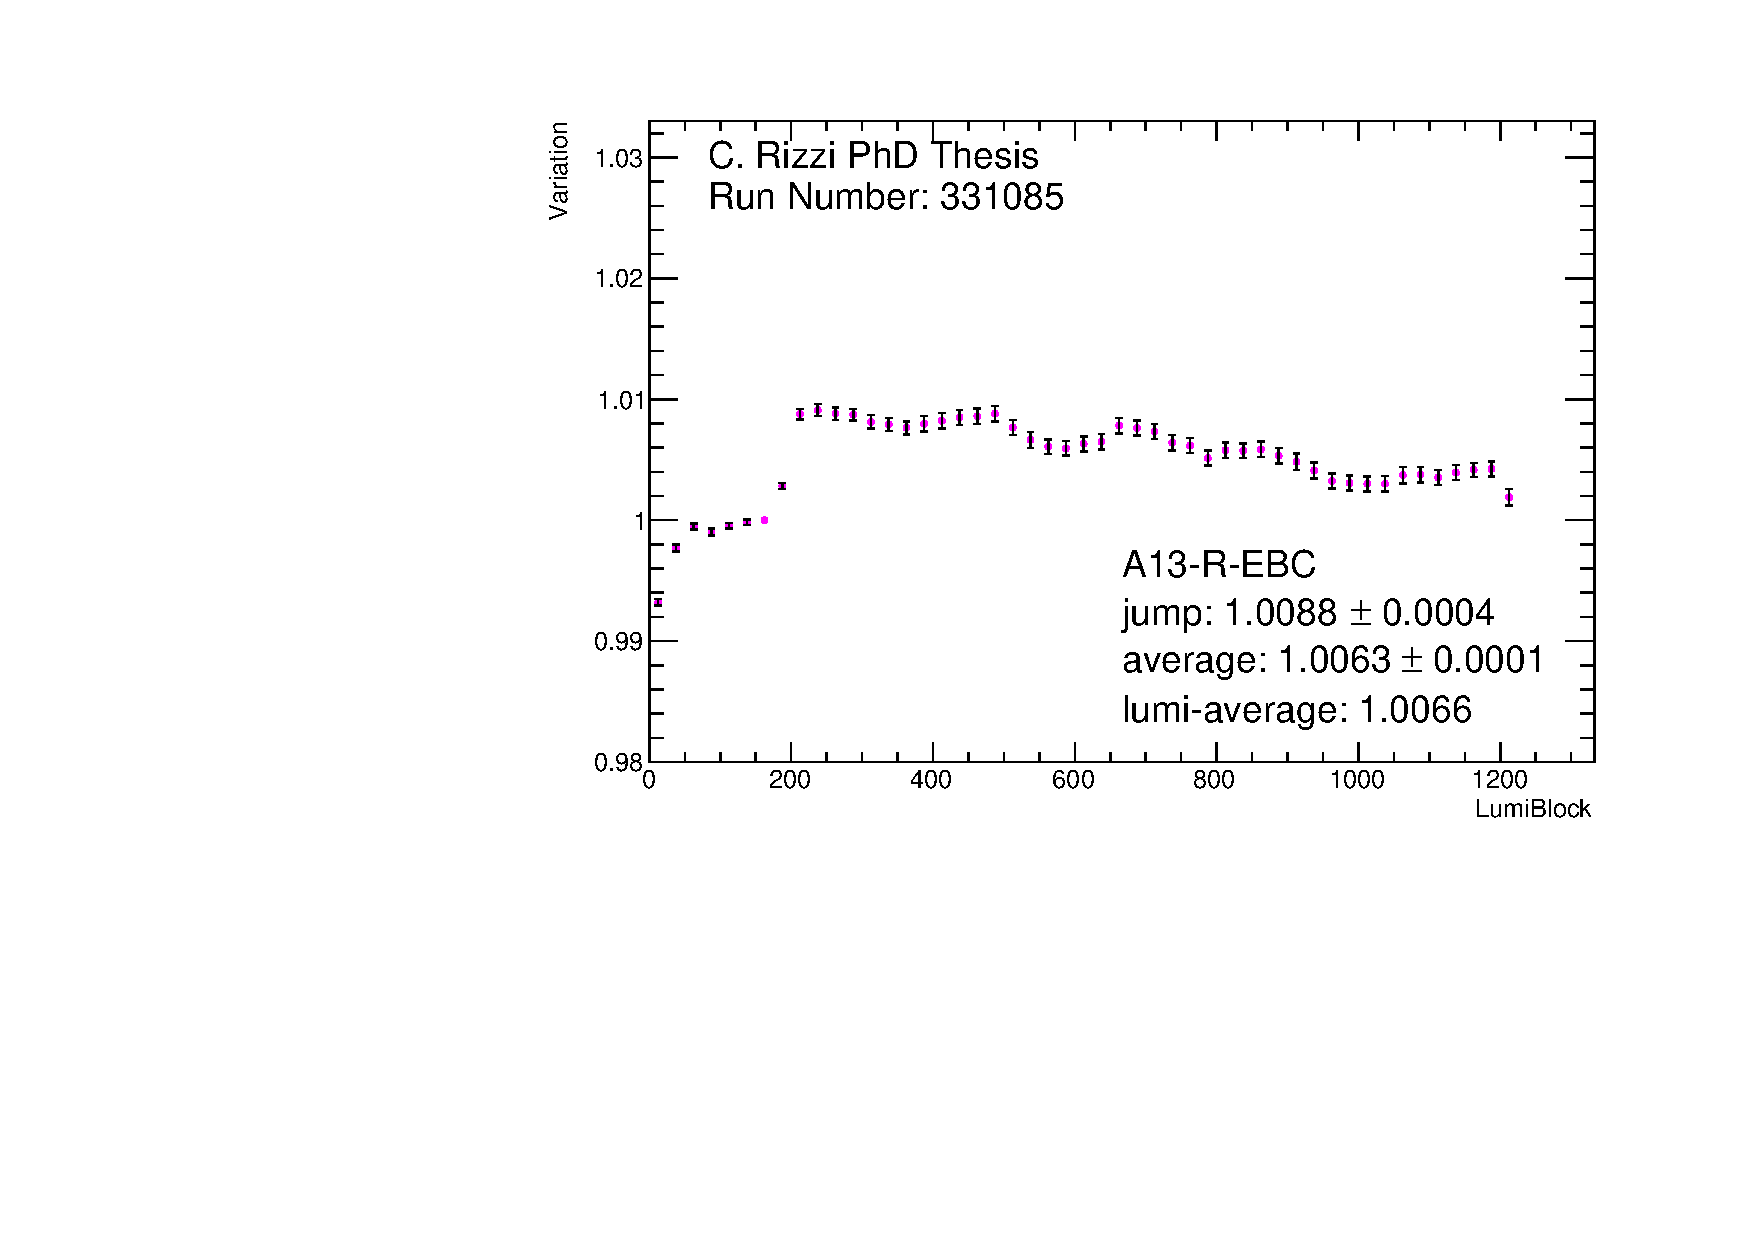
\includegraphics[width=0.45\textwidth]{figures/pmt_response/331085/variation_A13_R_EBC}\label{fig:app:variation_A13_R_EBC}}\\
\caption{\gls{pmt} response in cell A13 for the anchor run (run number 331085).}
\label{fig:apppmt:331085:variation_A13}
\end{figure}

\begin{figure}[htbp]
\centering
\subfigure{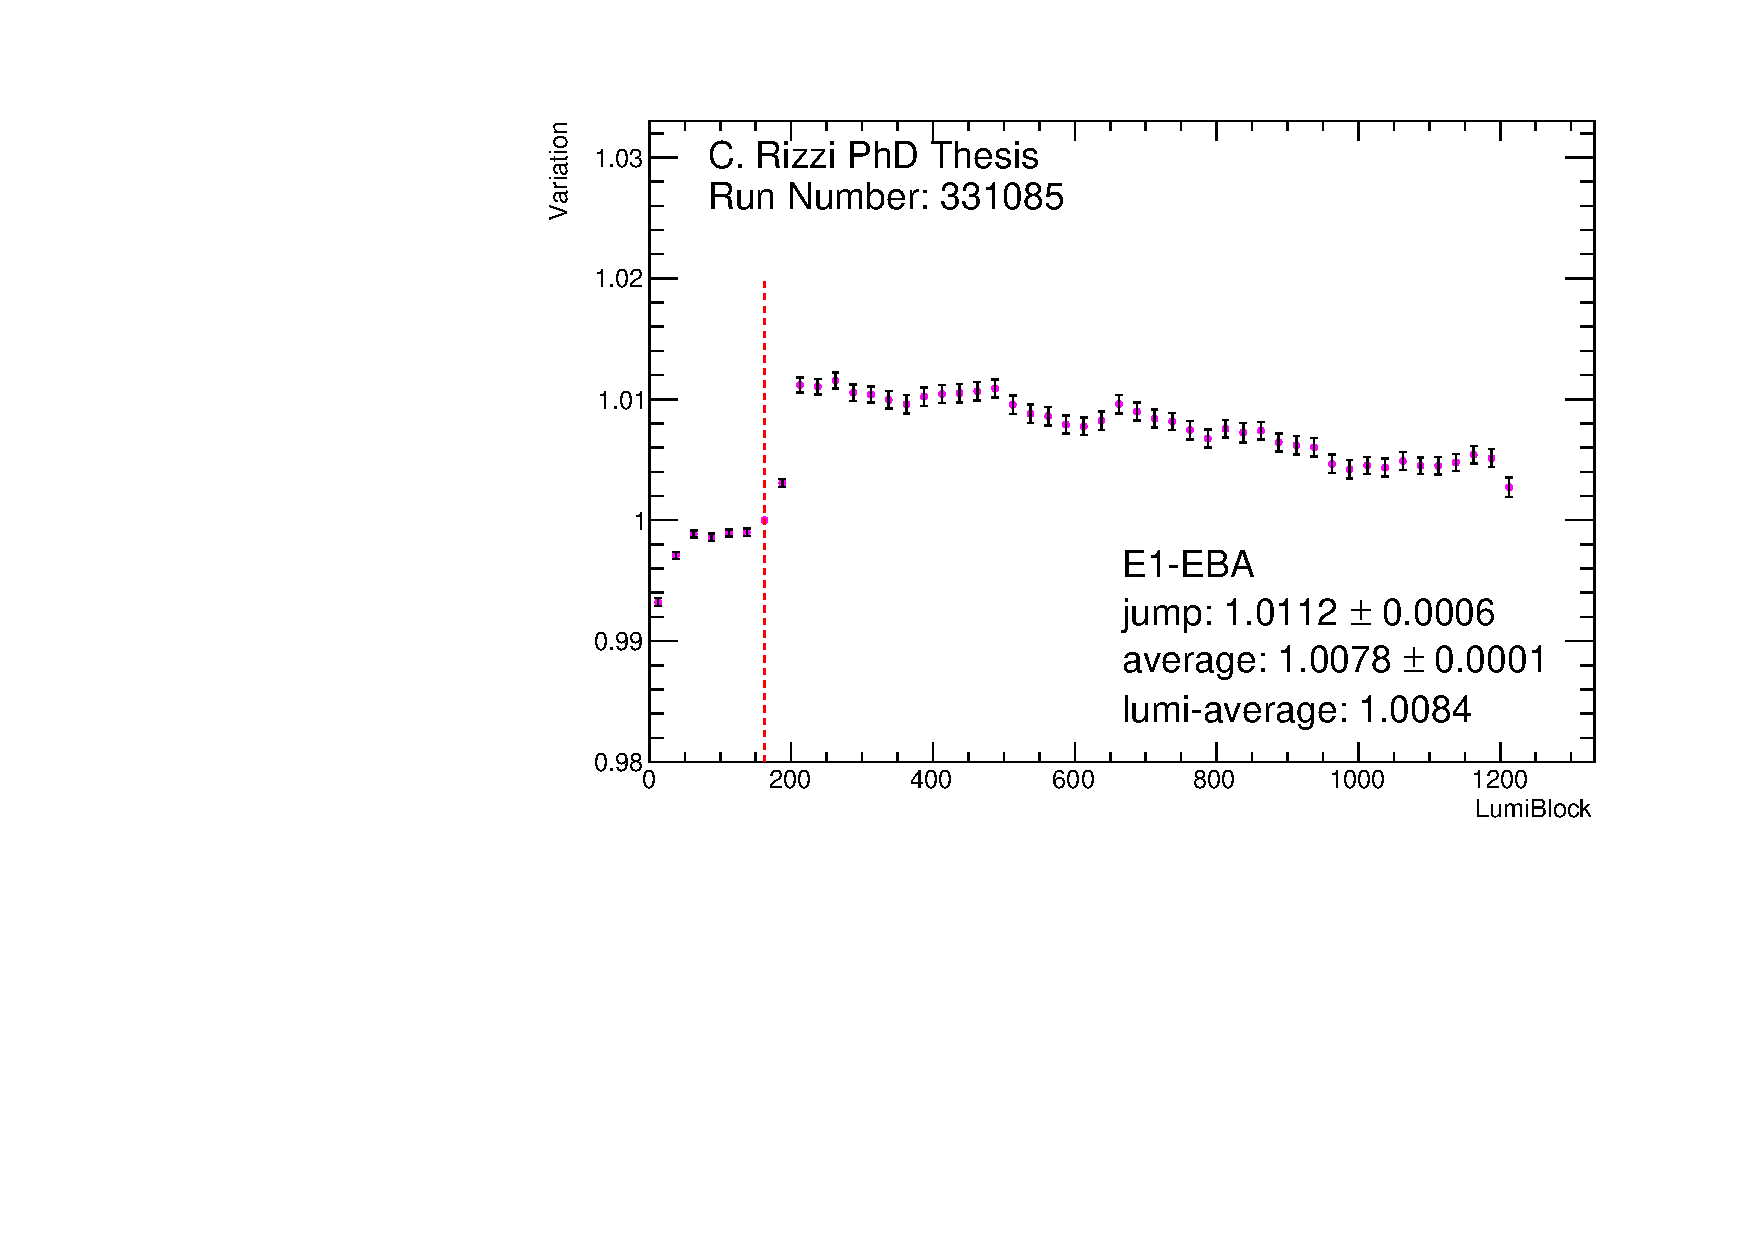
\includegraphics[width=0.45\textwidth]{figures/pmt_response/331085/variation_E1_EBA}\label{fig:app:variation_E1_EBA}}
\subfigure{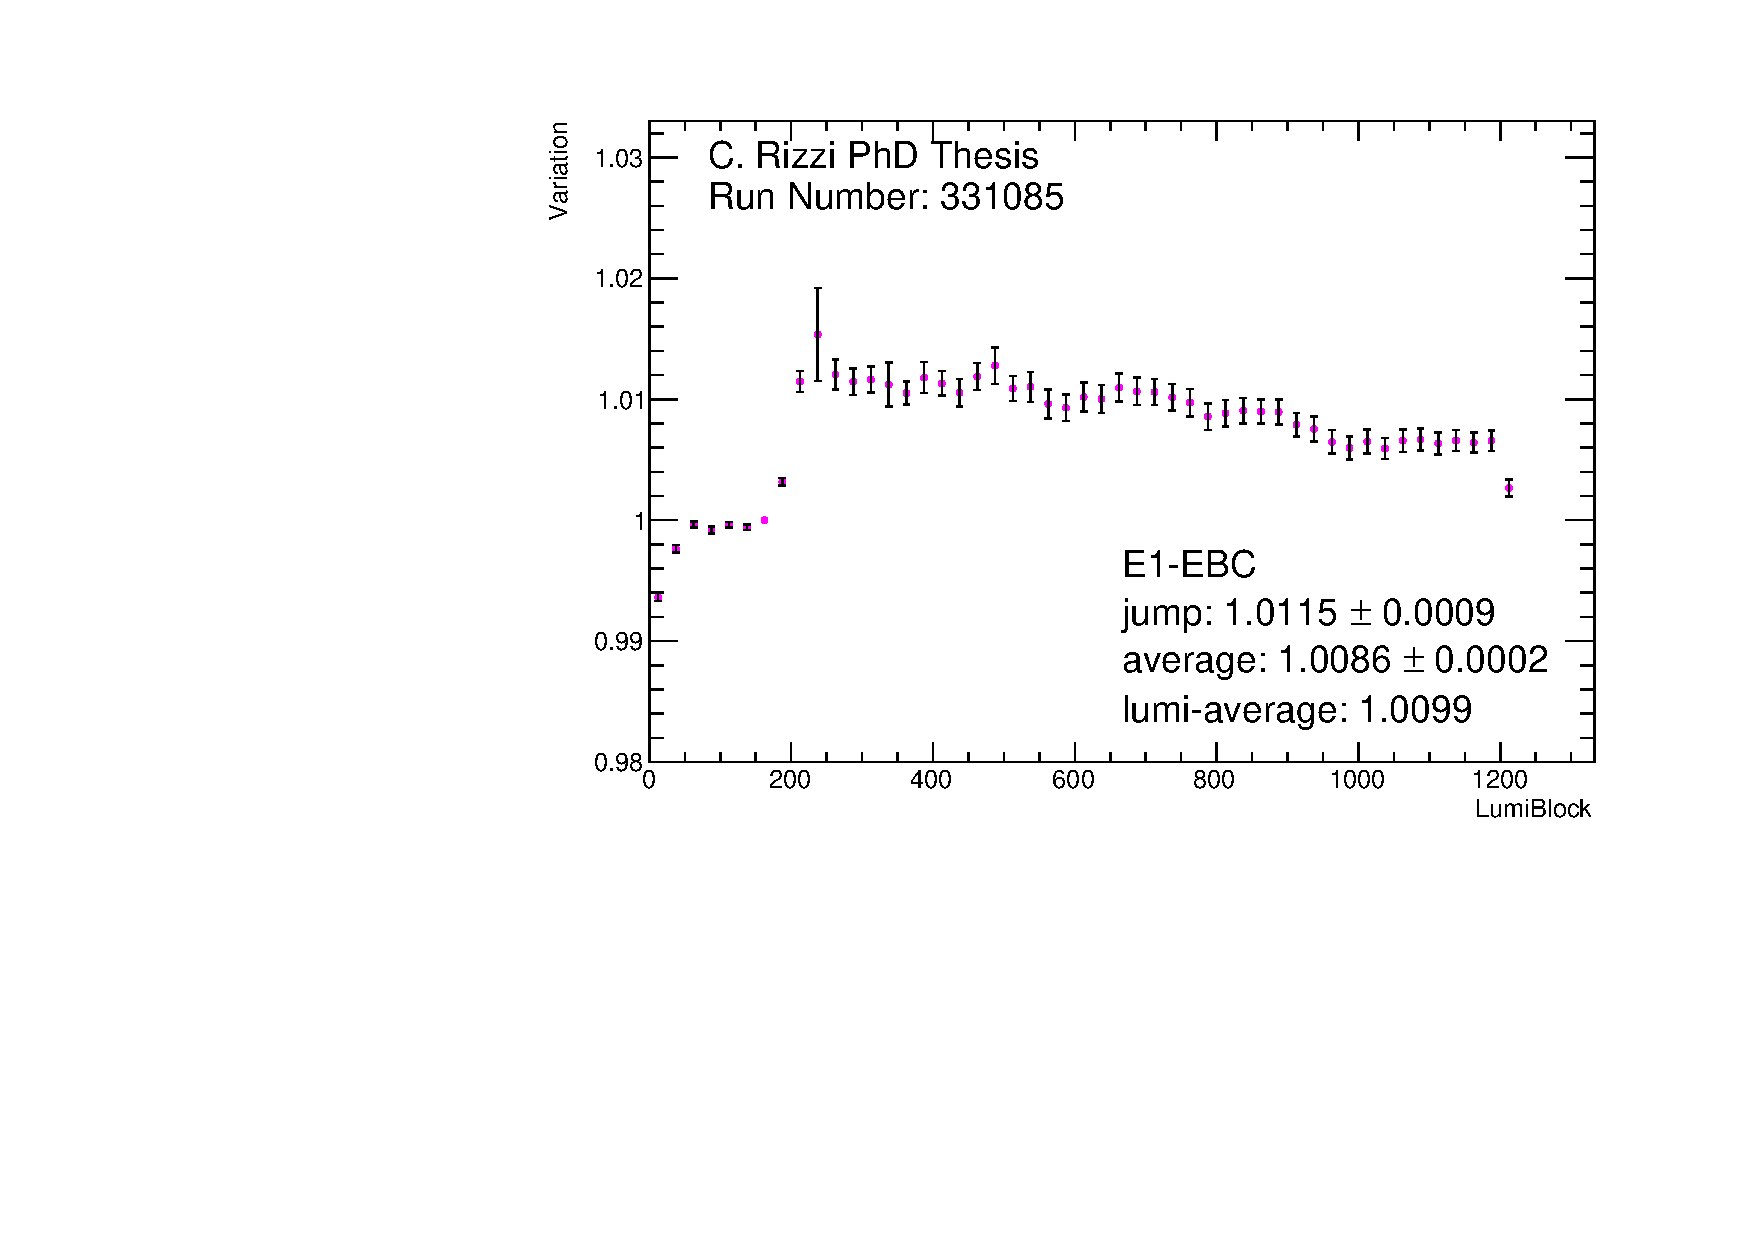
\includegraphics[width=0.45\textwidth]{figures/pmt_response/331085/variation_E1_EBC}\label{fig:app:variation_E1_EBC}}\\
\subfigure{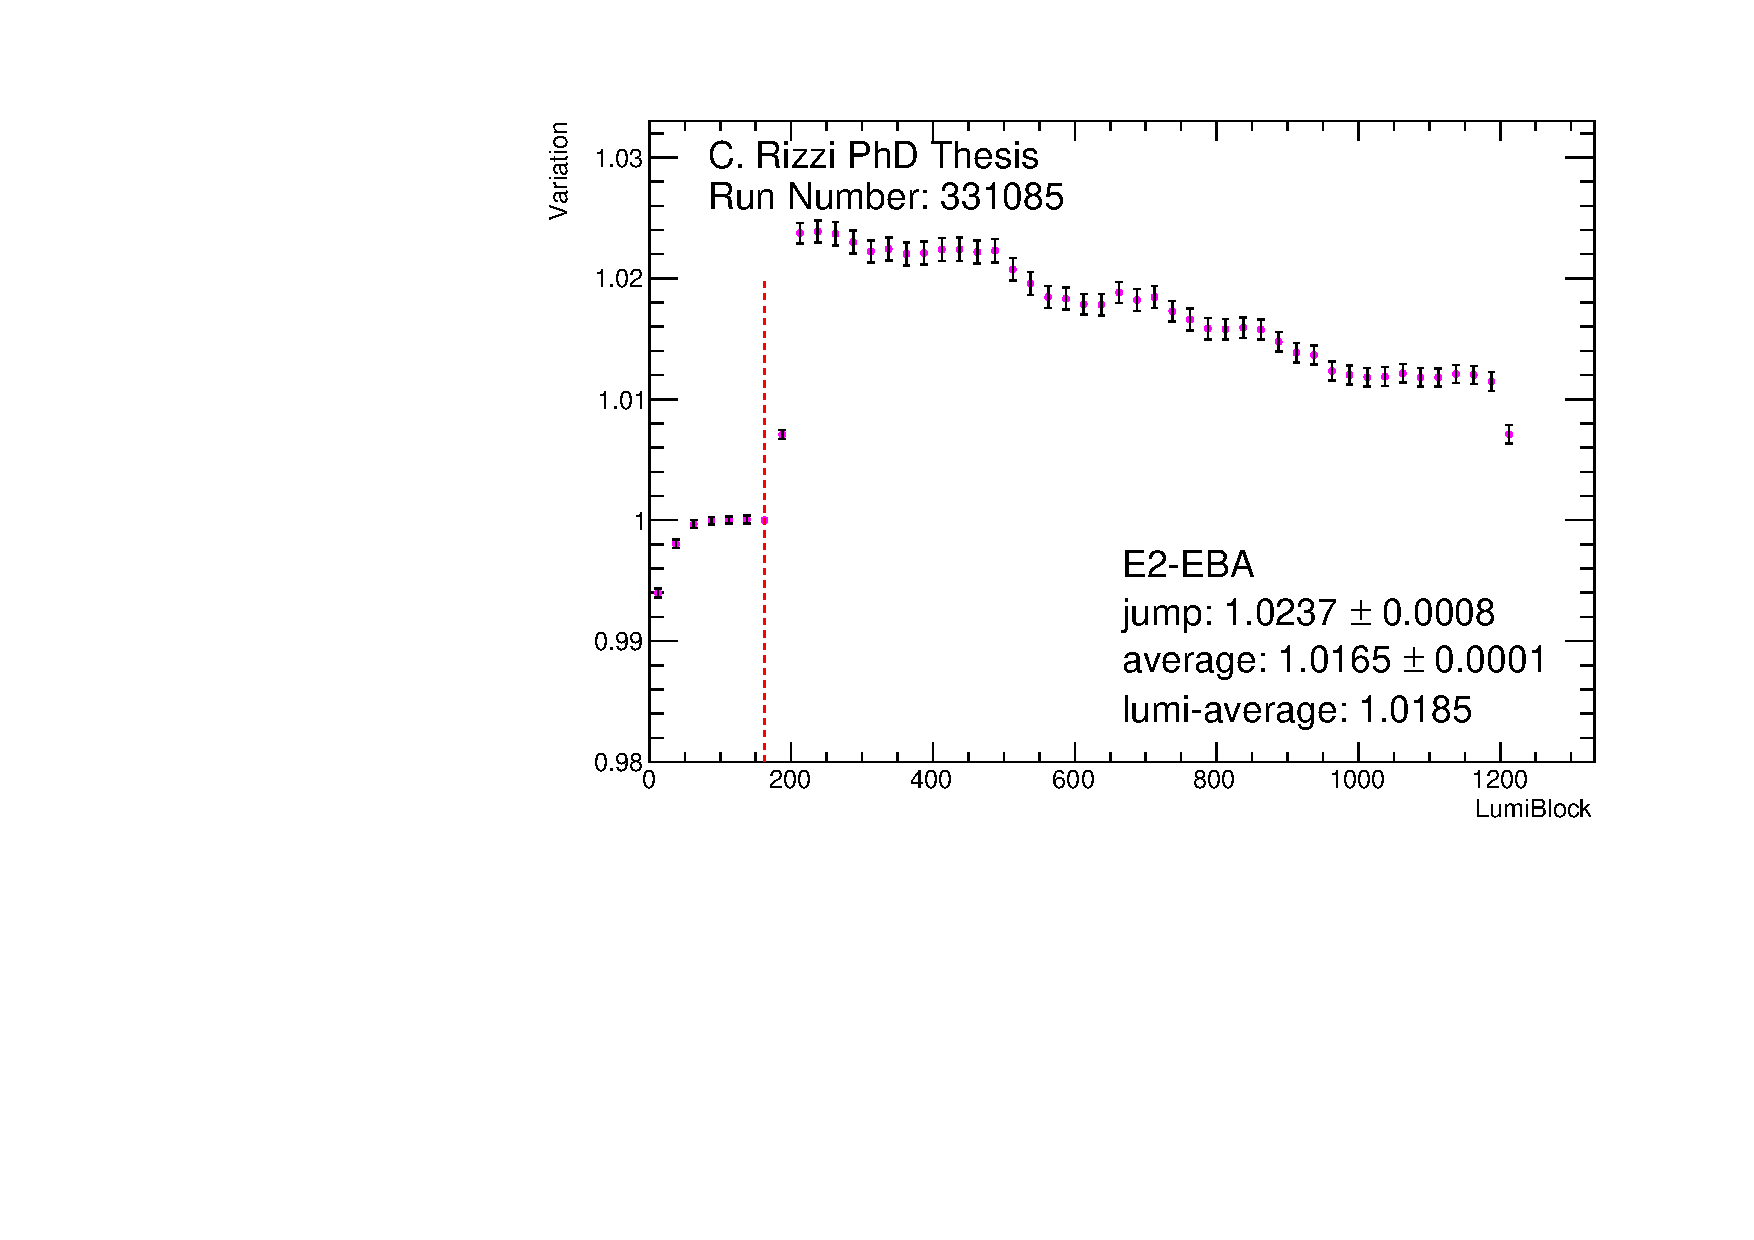
\includegraphics[width=0.45\textwidth]{figures/pmt_response/331085/variation_E2_EBA}\label{fig:app:variation_E2_EBA}}
\subfigure{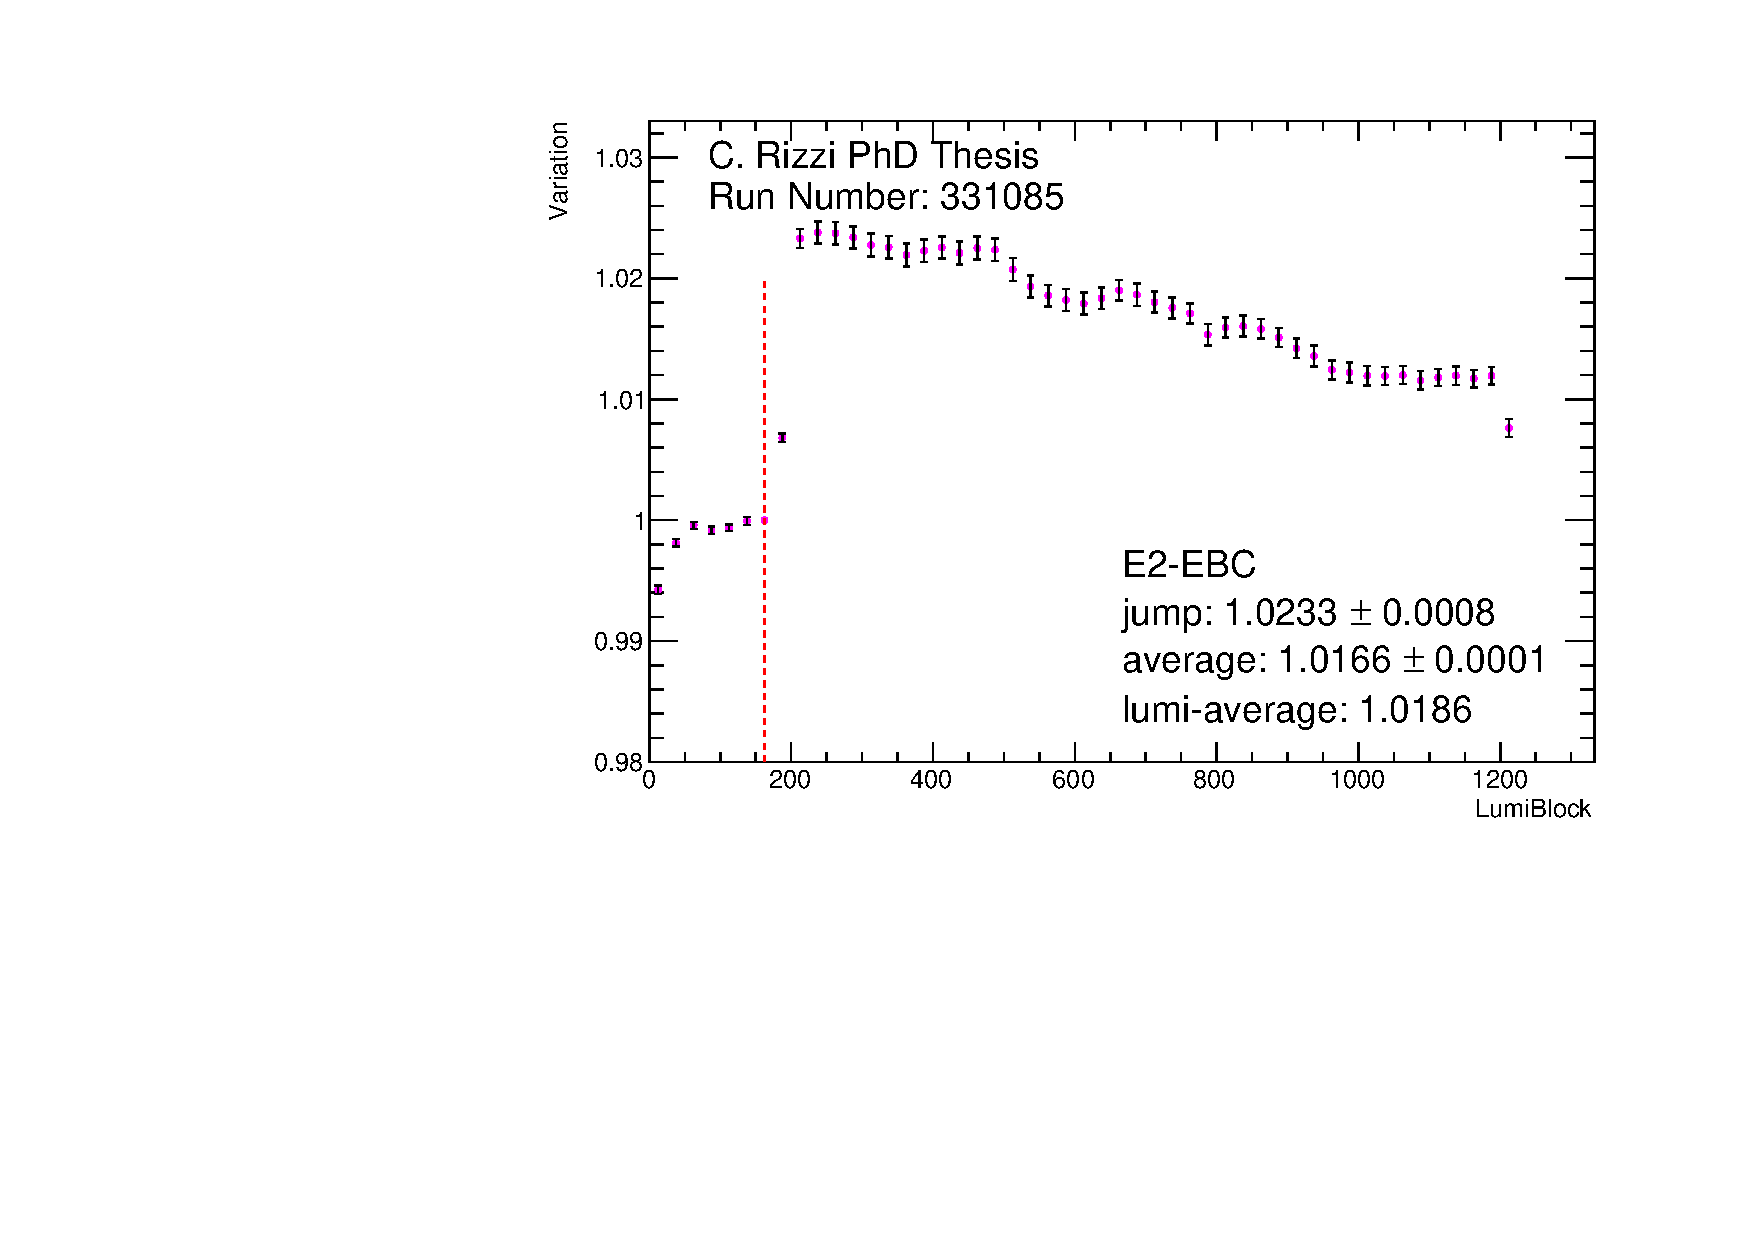
\includegraphics[width=0.45\textwidth]{figures/pmt_response/331085/variation_E2_EBC}\label{fig:app:variation_E2_EBC}}\\
\caption{\gls{pmt} response in cell E1 and E2 for the anchor run (run number 331085).}
\label{fig:apppmt:331085:variation_E1_E2}
\end{figure}

\begin{figure}[htbp]
\centering
\subfigure{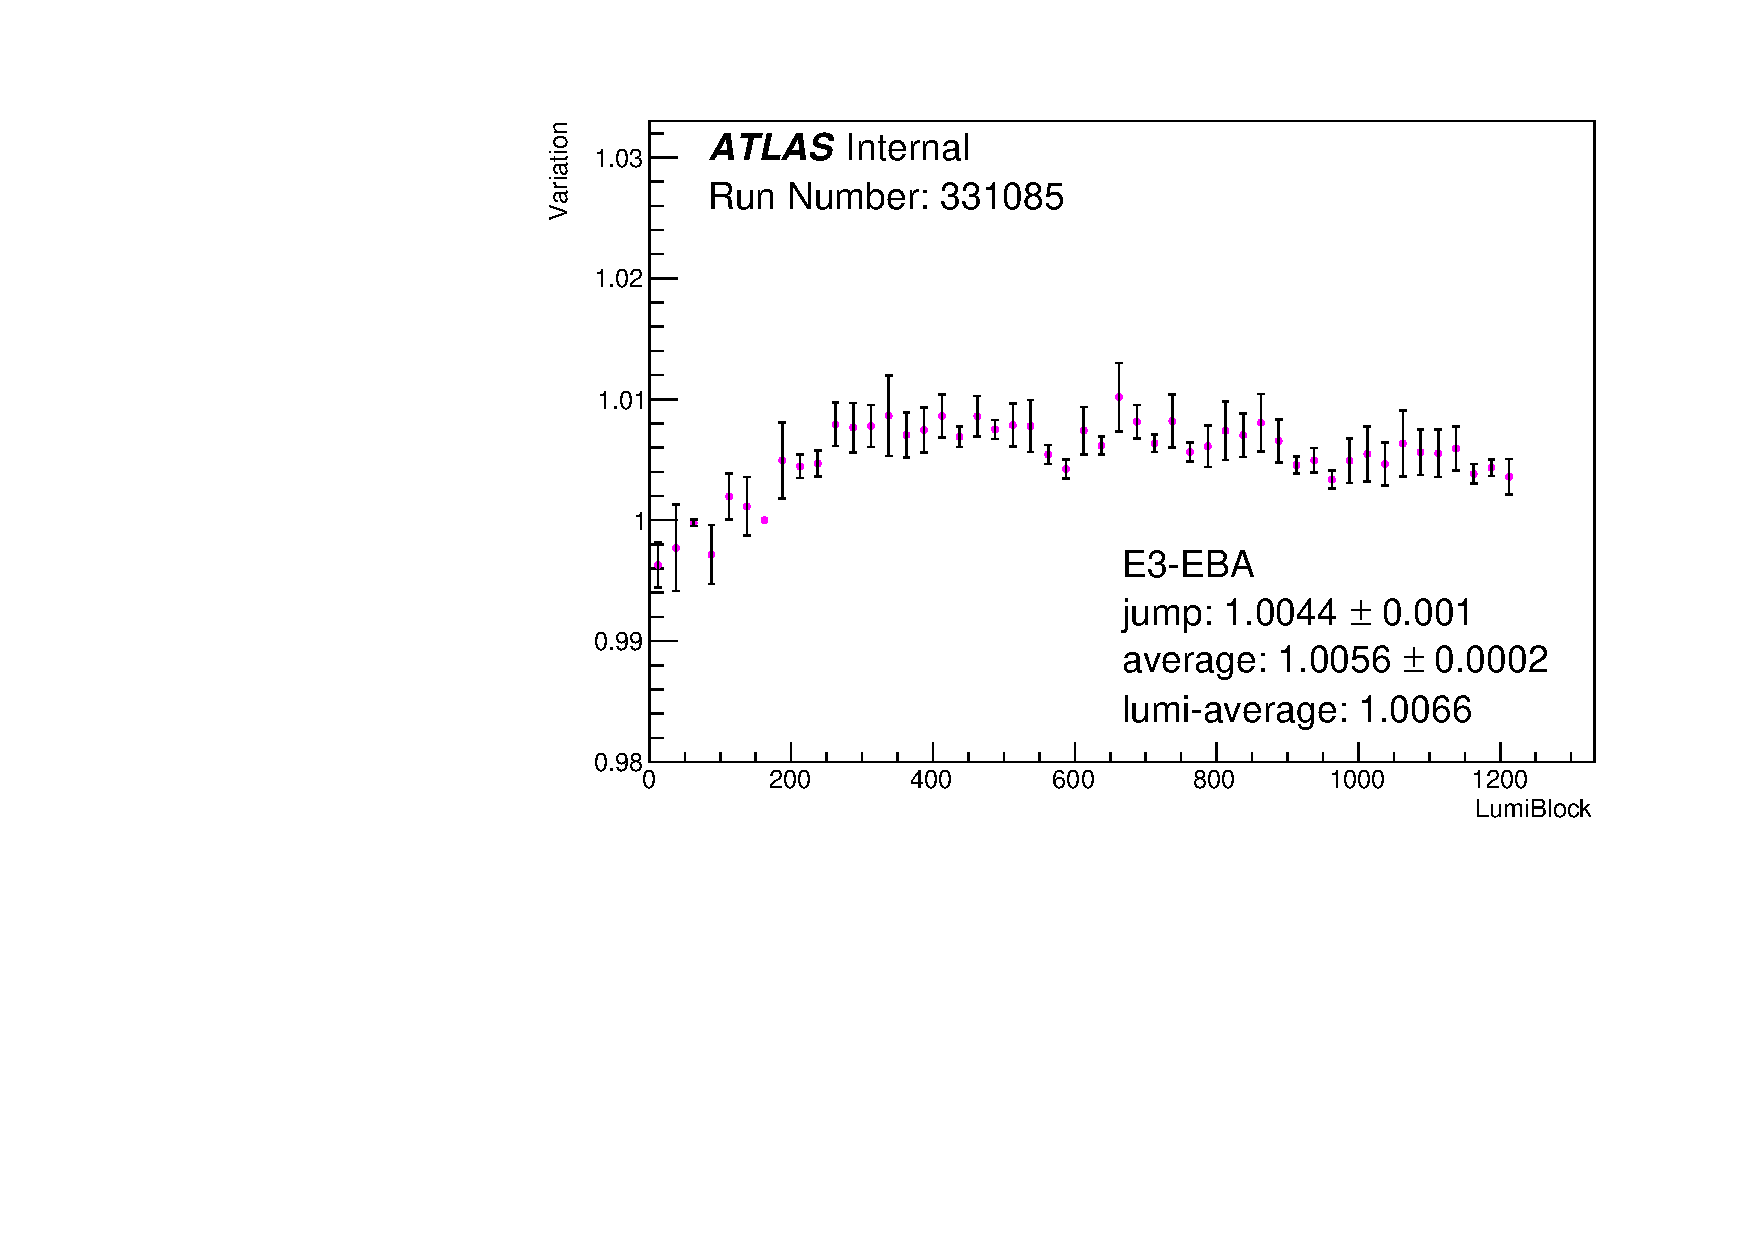
\includegraphics[width=0.45\textwidth]{figures/pmt_response/331085/variation_E3_EBA}\label{fig:app:variation_E3_EBA}}
\subfigure{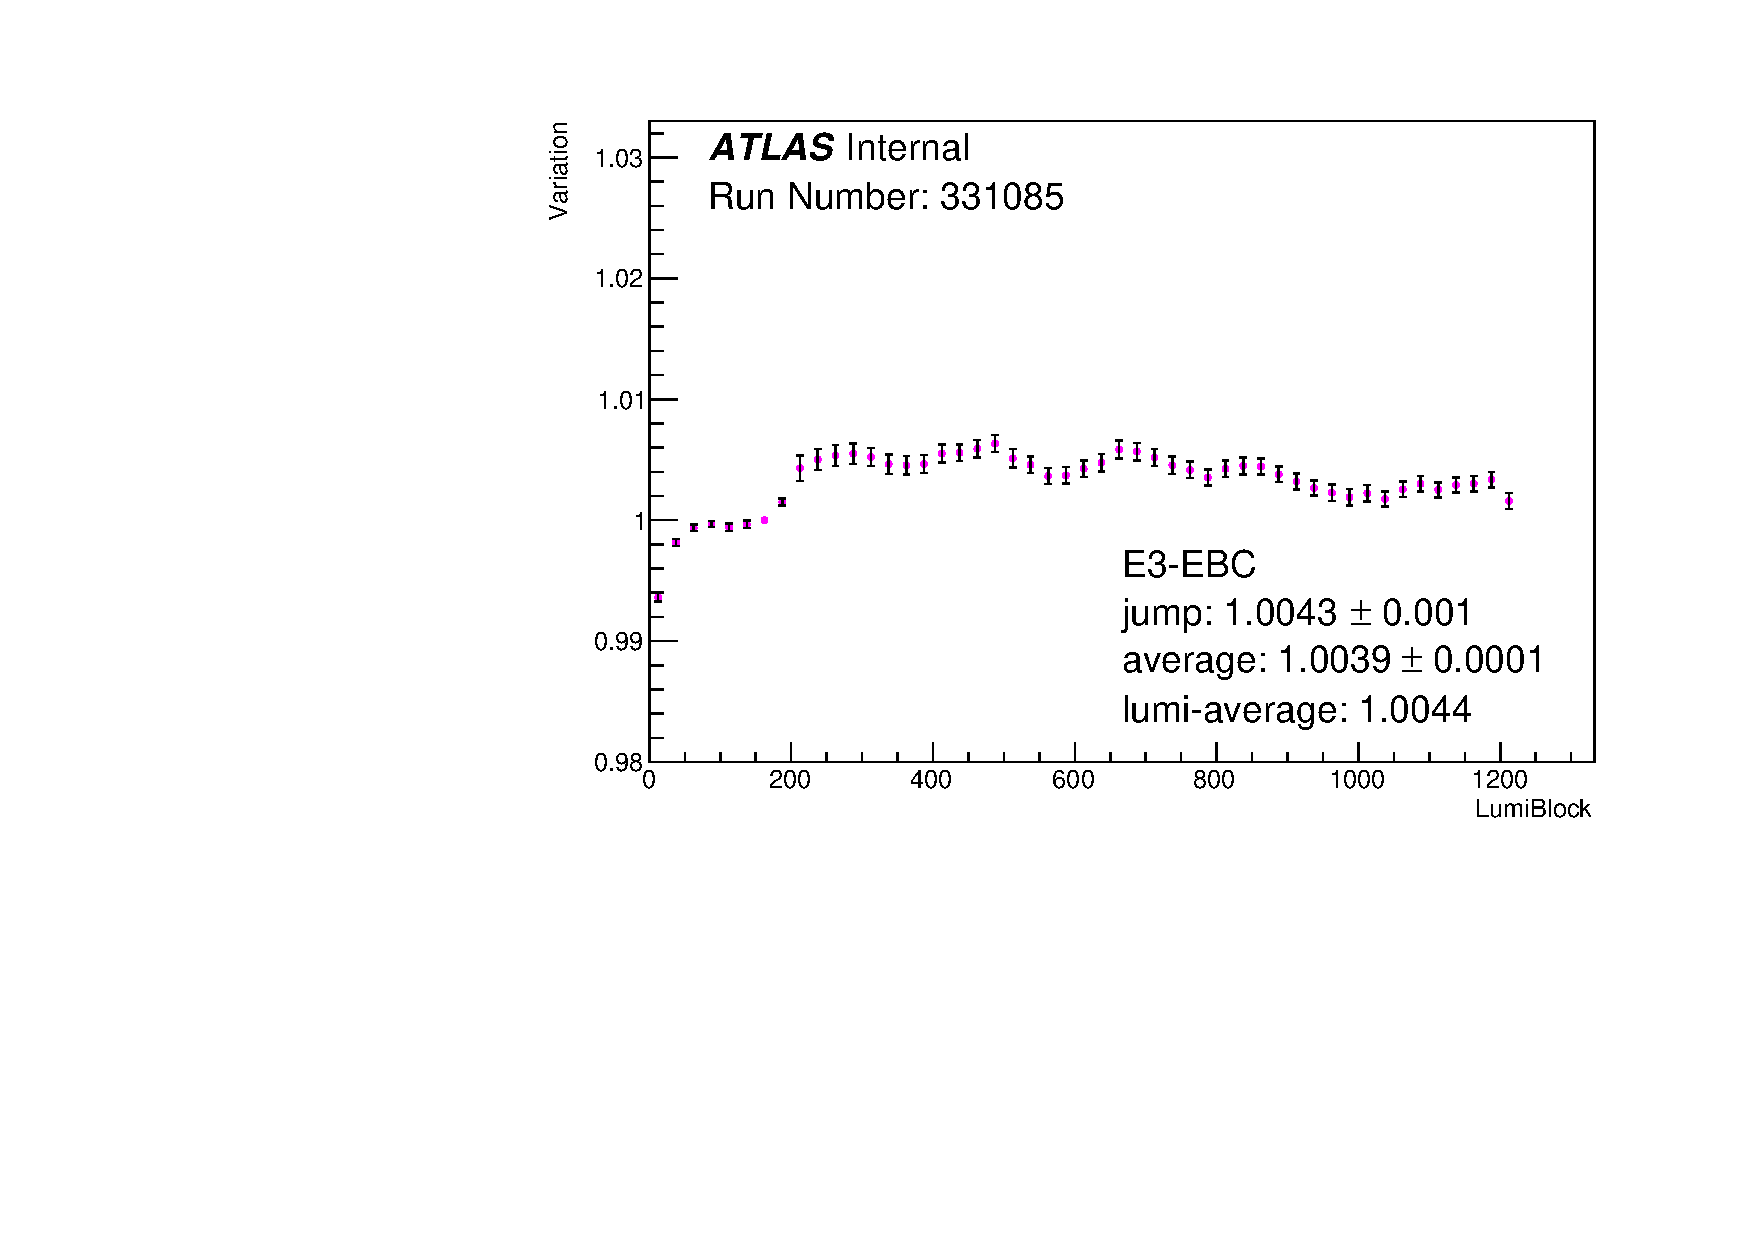
\includegraphics[width=0.45\textwidth]{figures/pmt_response/331085/variation_E3_EBC}\label{fig:app:variation_E3_EBC}}\\
\subfigure{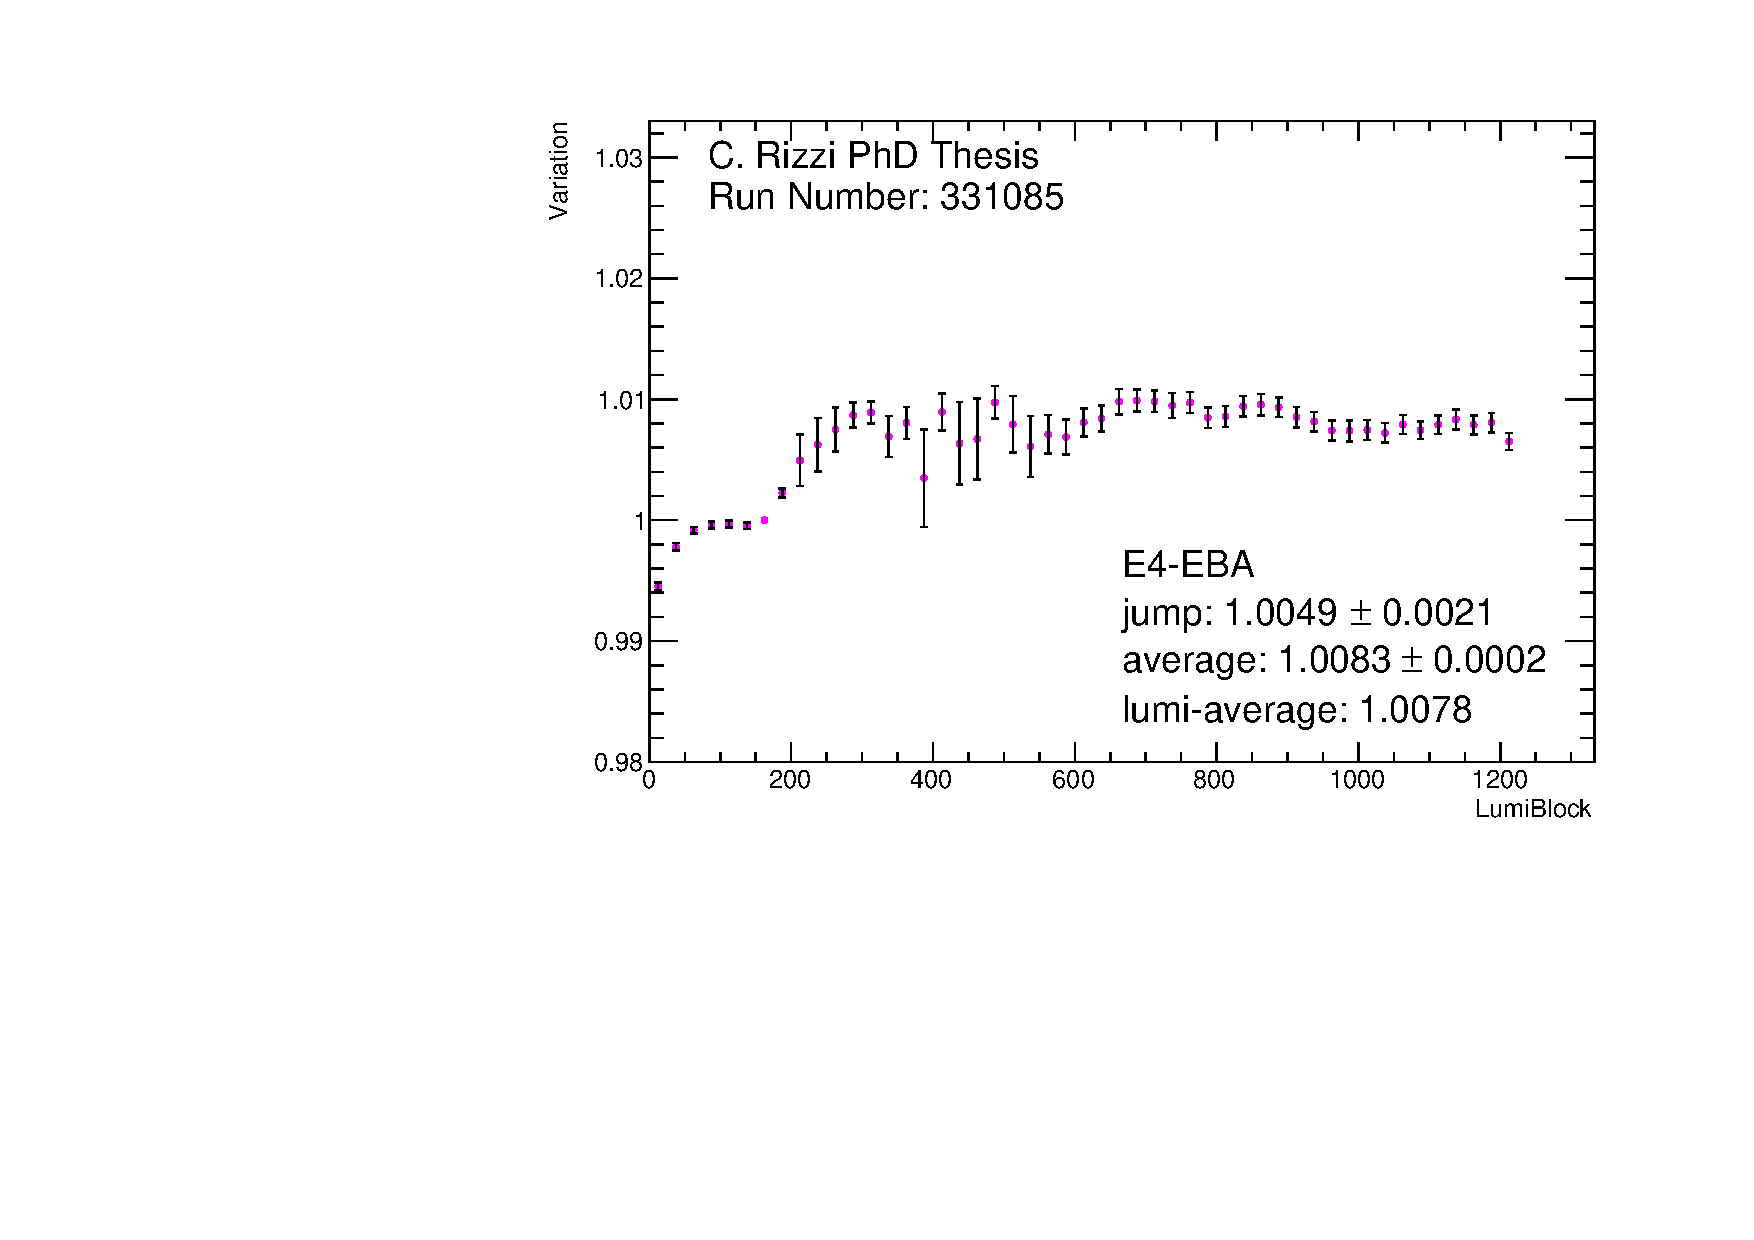
\includegraphics[width=0.45\textwidth]{figures/pmt_response/331085/variation_E4_EBA}\label{fig:app:variation_E4_EBA}}
\subfigure{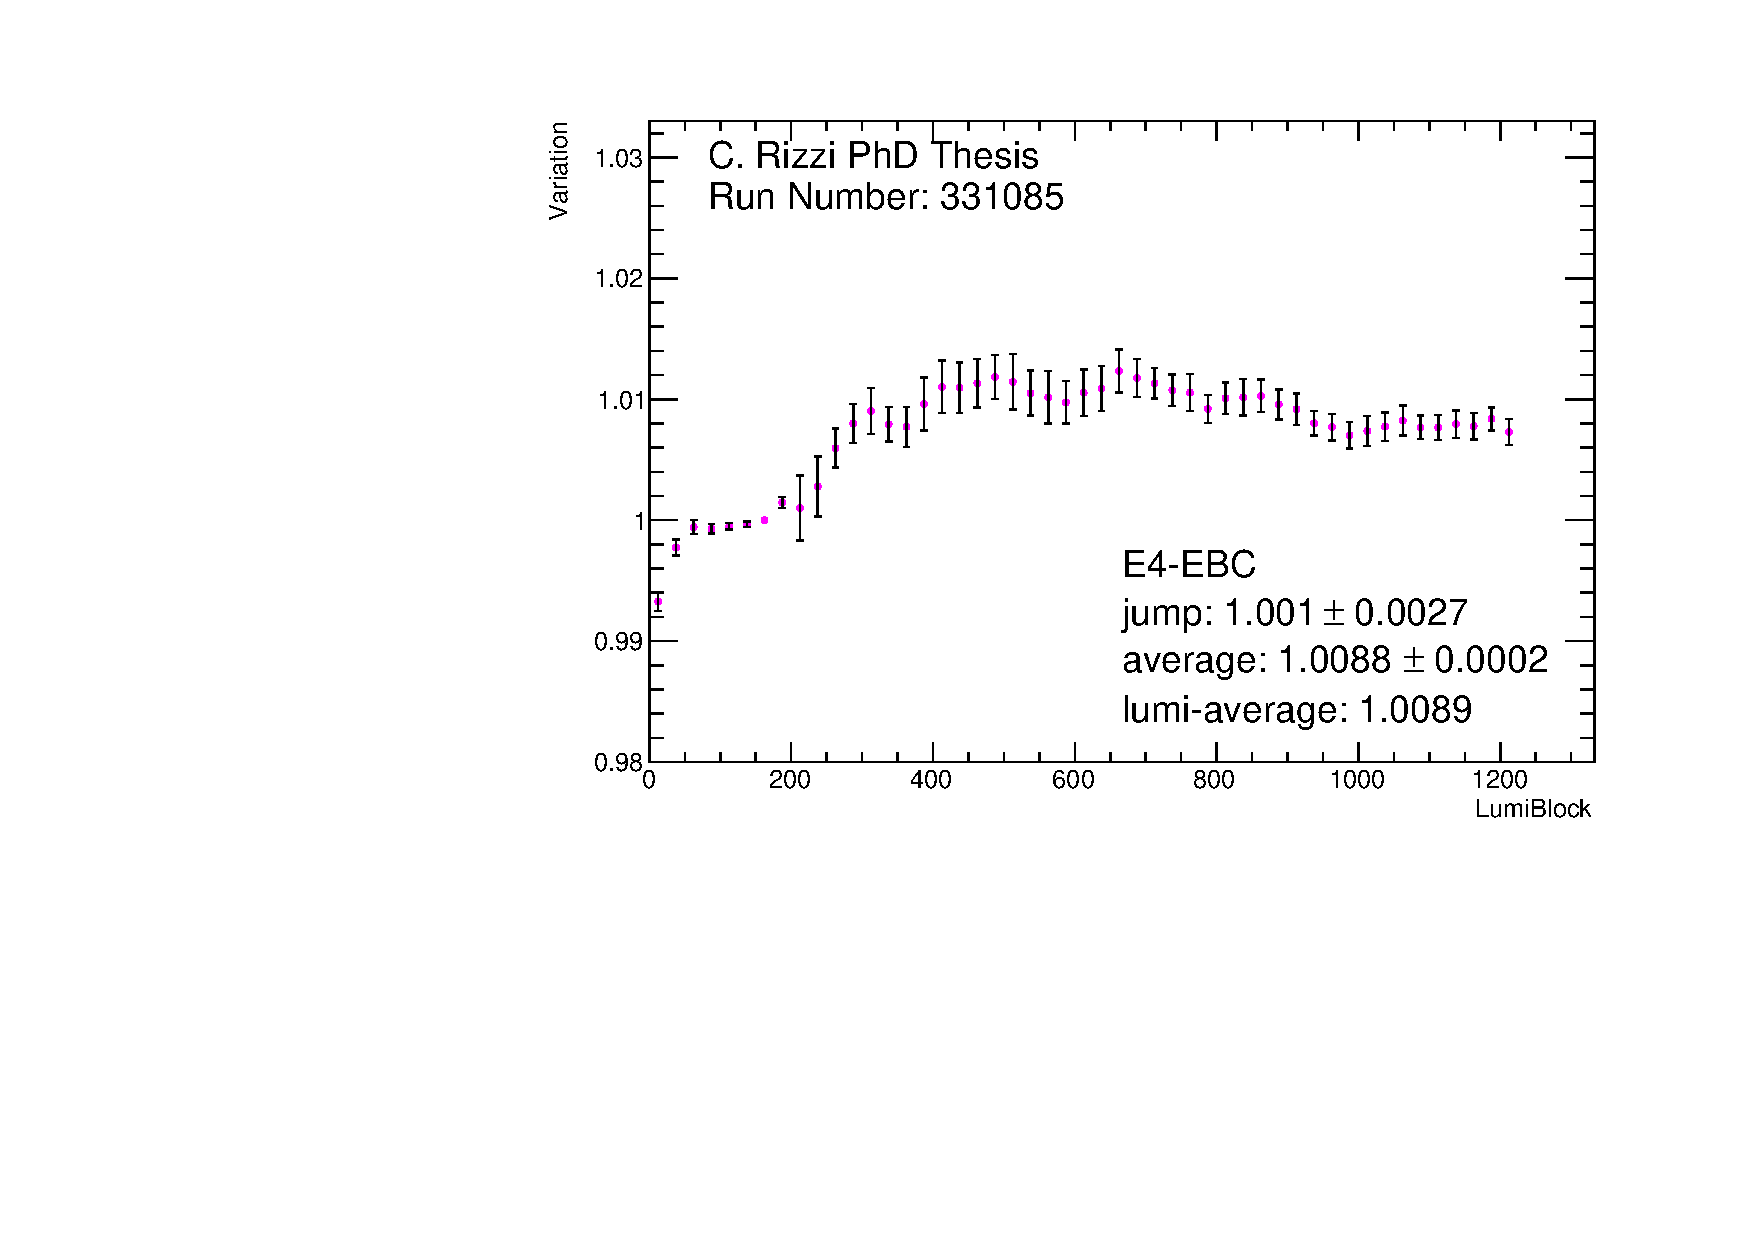
\includegraphics[width=0.45\textwidth]{figures/pmt_response/331085/variation_E4_EBC}\label{fig:app:variation_E4_EBC}}\\
\caption{\gls{pmt} response in cell E3 and E4 for the anchor run (run number 331085).}
\label{fig:apppmt:331085:variation_E3_E4}
\end{figure}

The \gls{pmt} non-linearity is quantified in three different ways, which in the Figures are labeled as:
\begin{description}
\item[Jump] Relative difference between the first group of \glspl{lub} after "stable beams" declaration that does not contain the 
\gls{lub} where "stable beams" is declared and the group of \glspl{lub} used as reference.
\item[Average] Average of the response after "stable beams" is declared until the end of the run, relative to the reference.
\item[Lumi-average] As above, but the average is weighted by the amount of luminosity collected in each group of \glspl{lub}.
\end{description}

 Equivalent studies on run 330875 show that for the low luminosity of the \gls{vdm} run there is no discontinuity in the 
 distribution of the \gls{pmt} response, and therefore no laser correction is needed for the \gls{vdm} run. 

\FloatBarrier


\section{Impact on calibration transfer uncertainty}

The change in the \gls{pmt} response with the increase in luminosity has a direct implication in the 
\gls{tilecal} luminosity measurement. 
In particular, it means that the increase in measured current with the increase in luminosity comes from 
two distinct factors:
\begin{itemize}
\item The actual increase in luminosity, i.e. having more particles traversing the detector.
\item The increase in \gls{pmt} response.
\end{itemize}

While the first bullet is the effect that we want to measure to provide a luminosity calibration, 
the second bullet has the effect of artificially increasing the \gls{tilecal} 
luminosity measurement. The value of the \gls{pmt} non-linearity measured in Section \ref{sec:app:pmtresponse} 
is used to correct for this undesired effect, with the net result of \gls{tilecal} providing a higher value 
for the luminosity measurement for the \gls{vdm} run, as schematically illustrated in Figure \ref{fig:apppmt:sketch}.


\begin{figure}[htbp]
\centering
\subfigure{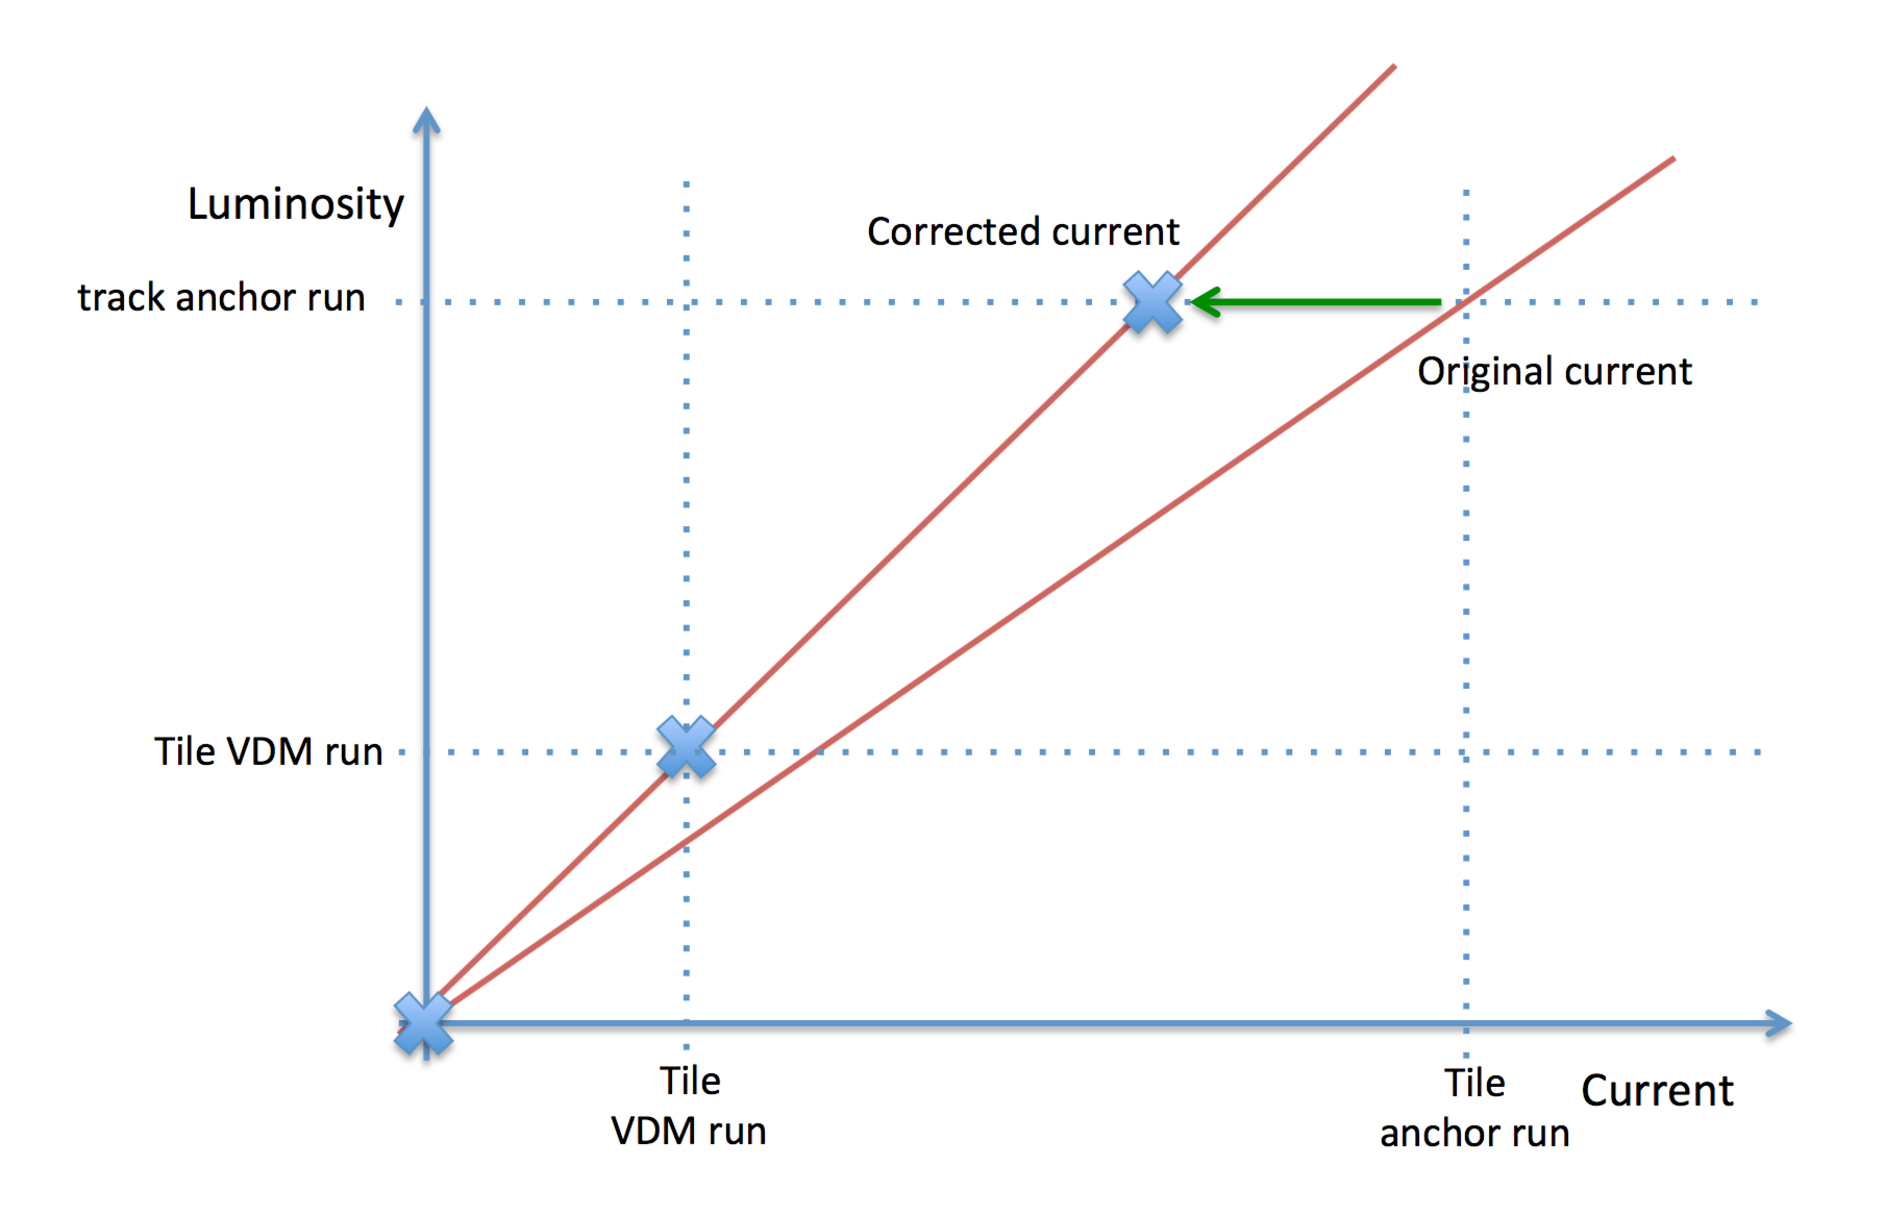
\includegraphics[width=0.65\textwidth]{figures/pmt_response/sketch.pdf}}
\caption{Schematic effect of the impact of the correction of the \gls{pmt} response on the \gls{tilecal} luminosity measurement.}
\label{fig:apppmt:sketch}
\end{figure}


Figures \ref{fig:app:vdm_rel_track_mod_EBA} and \ref{fig:app:vdm_rel_track_mod_EBC} 
show the effect of the correction derived for the cell families used in the computation of the 
calibration transfer uncertainty, for the A side and C side respectively. 



\begin{figure}[htbp]
\centering
\subfigure{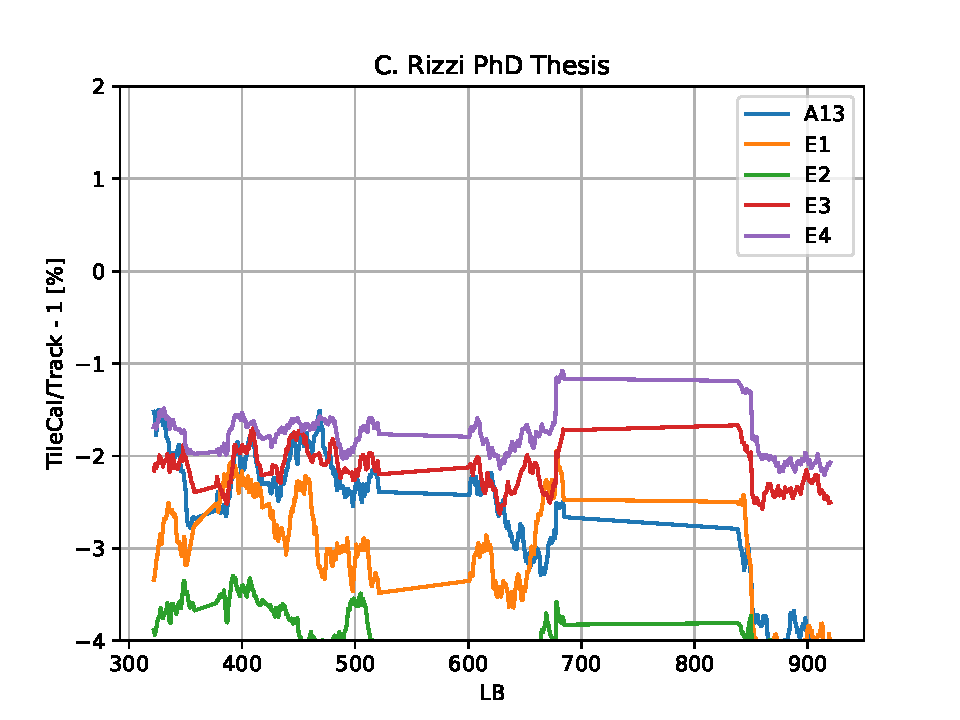
\includegraphics[width=0.48\textwidth]{figures/pmt_response/results/vdm_noPMTcorr_rel_track_mod_EBA.pdf}\label{fig:app:vdm_noPMTcorr_rel_track_mod_EBA}}
\subfigure{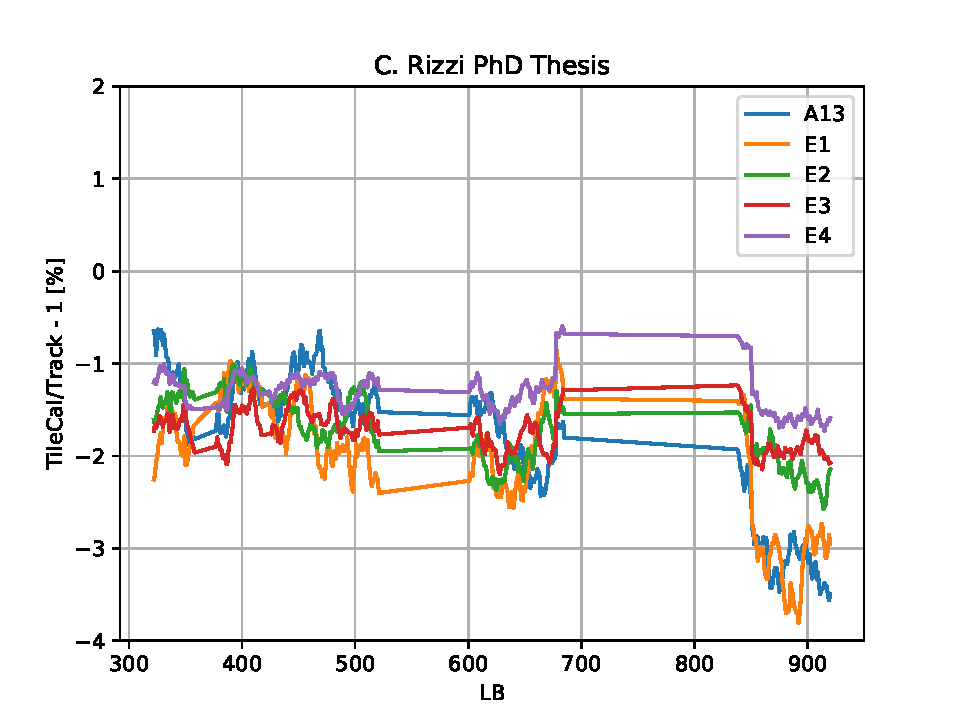
\includegraphics[width=0.48\textwidth]{figures/pmt_response/results/vdm_jump_rel_track_mod_EBA.pdf}\label{fig:app:vdm_jump_rel_track_mod_EBA}}\\
\subfigure{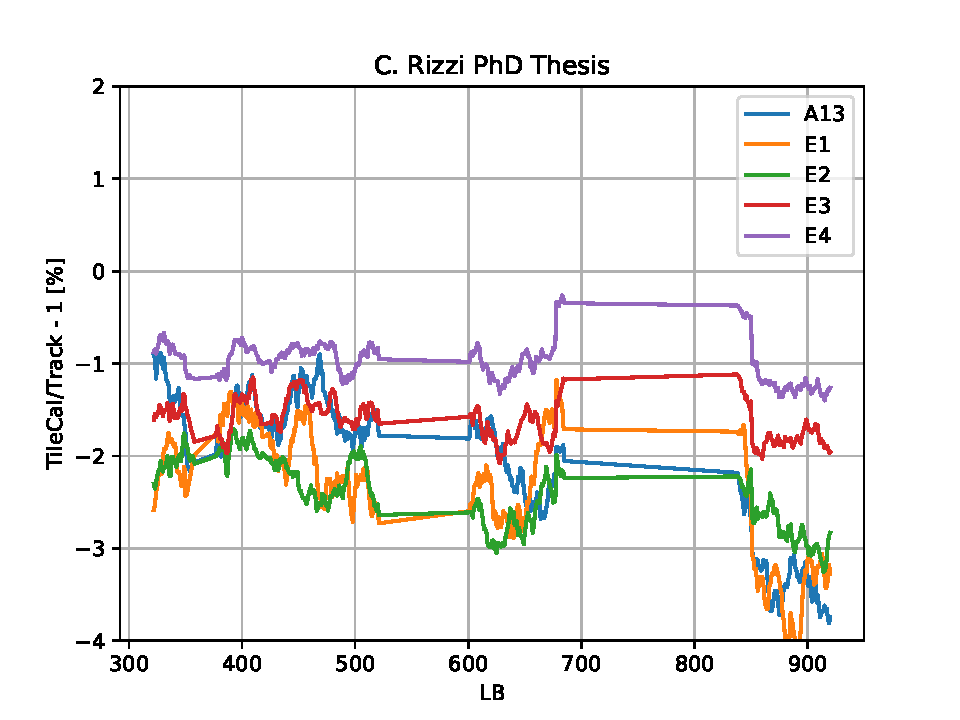
\includegraphics[width=0.48\textwidth]{figures/pmt_response/results/vdm_ave_rel_track_mod_EBA.pdf}\label{fig:app:vdm_ave_rel_track_mod_EBA}}
\subfigure{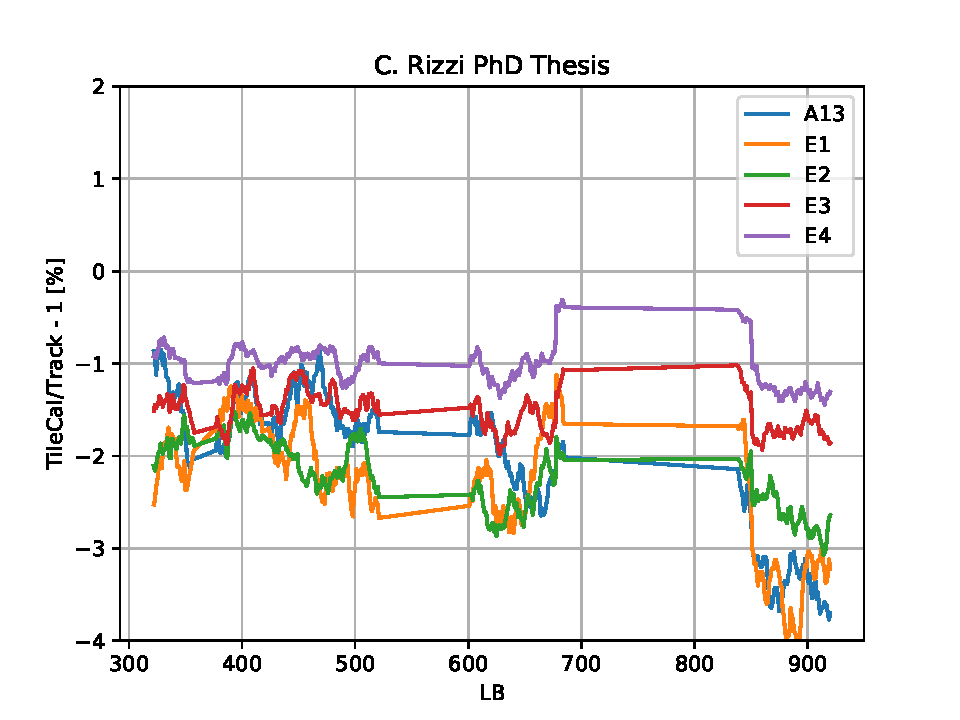
\includegraphics[width=0.48\textwidth]{figures/pmt_response/results/vdm_lumiAve_rel_track_mod_EBA.pdf}\label{fig:app:vdm_lumiAve_rel_track_mod_EBA}}\\
\caption{Fractional difference between the \gls{tilecal} and Tracking luminosities for the \gls{vdm} run
\subref{fig:app:vdm_noPMTcorr_rel_track_mod_EBA} without any laser correction, 
\subref{fig:app:vdm_jump_rel_track_mod_EBA} with the "jump" correction,
\subref{fig:app:vdm_ave_rel_track_mod_EBA} with the "average" correction and 
\subref{fig:app:vdm_lumiAve_rel_track_mod_EBA} with the "lumi-average" correction.
Only cell families from EBA are used. 
}
\label{fig:app:vdm_rel_track_mod_EBA}
\end{figure}


\begin{figure}[htbp]
\centering
\subfigure{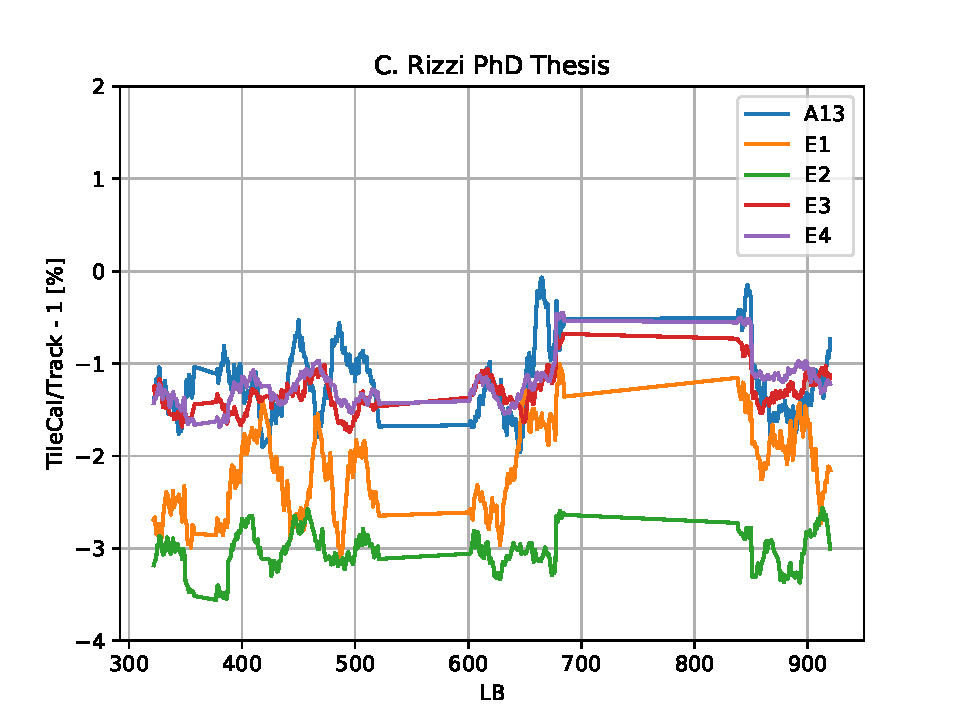
\includegraphics[width=0.48\textwidth]{figures/pmt_response/results/vdm_noPMTcorr_rel_track_mod_EBC.pdf}\label{fig:app:vdm_noPMTcorr_rel_track_mod_EBC}}
\subfigure{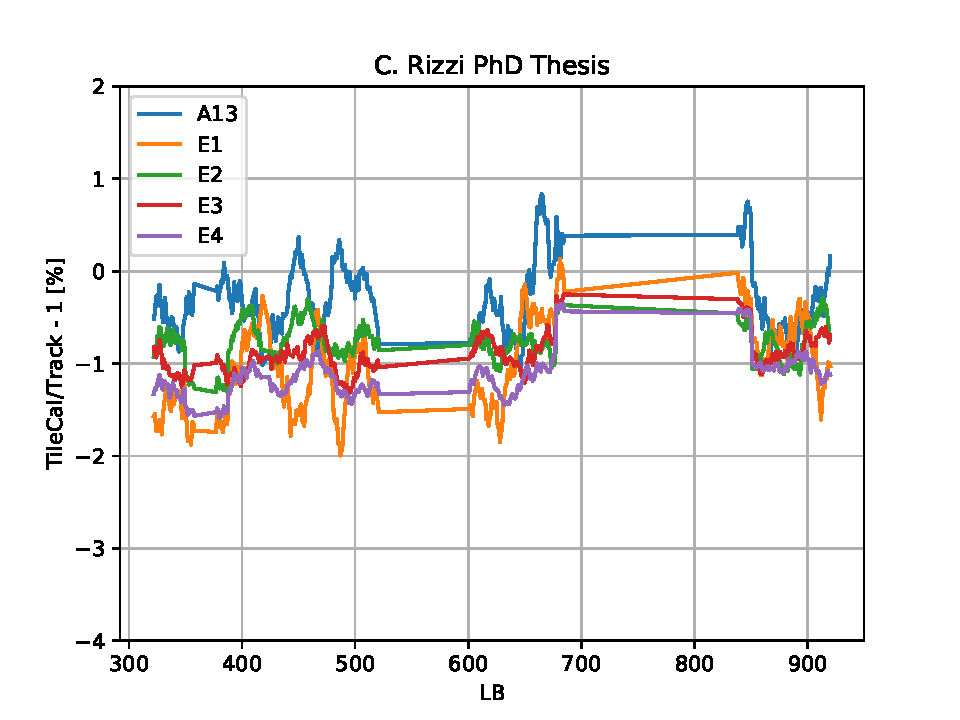
\includegraphics[width=0.48\textwidth]{figures/pmt_response/results/vdm_jump_rel_track_mod_EBC.pdf}\label{fig:app:vdm_jump_rel_track_mod_EBC}}\\
\subfigure{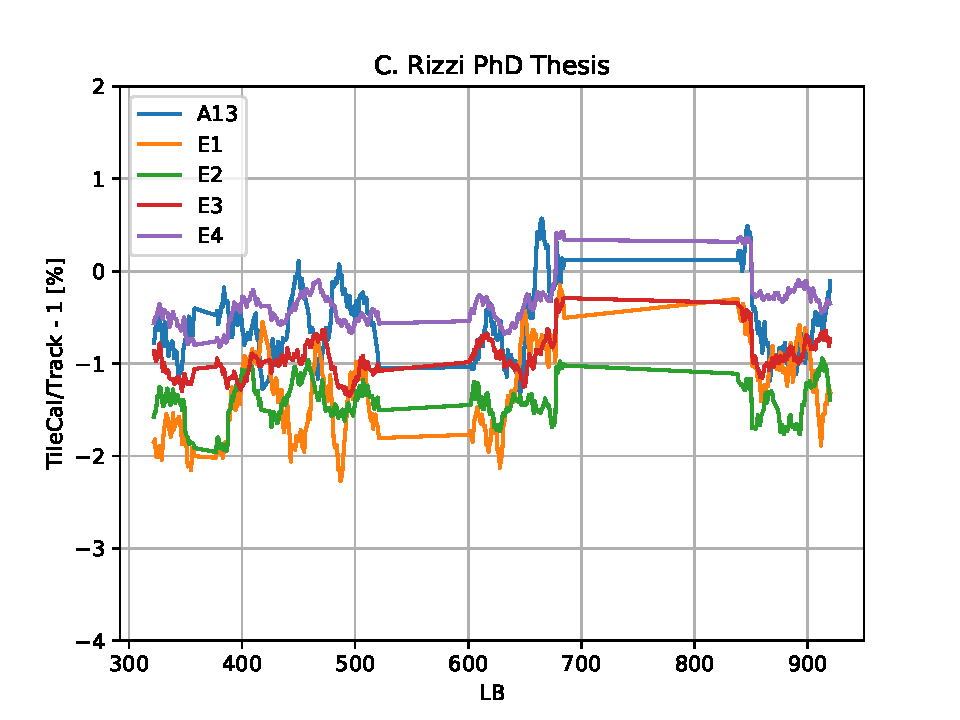
\includegraphics[width=0.48\textwidth]{figures/pmt_response/results/vdm_ave_rel_track_mod_EBC.pdf}\label{fig:app:vdm_ave_rel_track_mod_EBC}}
\subfigure{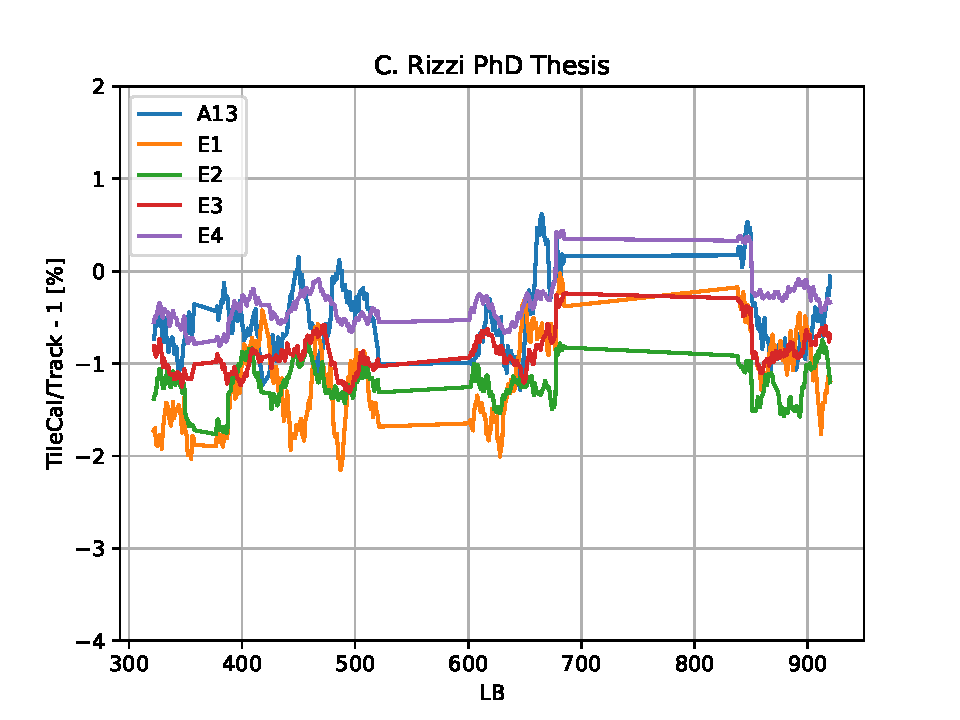
\includegraphics[width=0.48\textwidth]{figures/pmt_response/results/vdm_lumiAve_rel_track_mod_EBC.pdf}\label{fig:app:vdm_lumiAve_rel_track_mod_EBC}}\\
\caption{Fractional difference between the \gls{tilecal} and Tracking luminosities for the \gls{vdm} run
\subref{fig:app:vdm_noPMTcorr_rel_track_mod_EBC} without any laser correction, 
\subref{fig:app:vdm_jump_rel_track_mod_EBC} with the "jump" correction,
\subref{fig:app:vdm_ave_rel_track_mod_EBC} with the "average" correction and 
\subref{fig:app:vdm_lumiAve_rel_track_mod_EBC} with the "lumi-average" correction.
Only cell families from EBC are used. 
}
\label{fig:app:vdm_rel_track_mod_EBC}
\end{figure}

To quantify the improvement provided by the laser corrections, we can compute the integrated luminosity over the whole 
\gls{vdm} run for the \gls{tilecal} cell families and compare it to the integrated luminosity from the tracking system; 
this is shown in Figure \ref{fig:apppmt:totallumi}. 
The average relative difference between \gls{tilecal} and Tracking luminosity, averaged over all 
the considered cell families, results to be:
\begin{itemize}
\item no \gls{pmt} correction: 2.19\%,
\item jump: 1.19 \%,
\item average: 1.32 \%,
\item Lumi-average: 1.25 \%.
\end{itemize}
\noindent We can see that the inclusion of the laser corrections reduces the uncertainty by about 1\% absolute.

\begin{figure}[htbp]
\centering
\subfigure{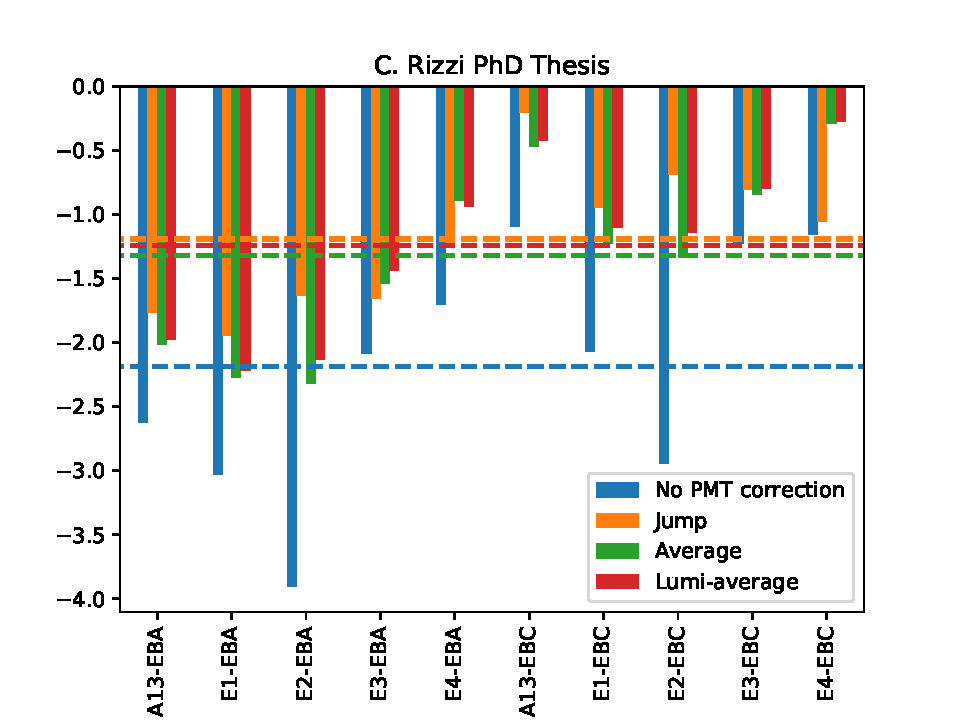
\includegraphics[width=0.80\textwidth]{figures/pmt_response/lumi_integral.pdf}}
\caption{Relative difference in total integrated luminosity for the \gls{vdm} run for the different types of 
\gls{pmt} corrections. The dashed line shows the average of the difference over all the cell families considered, which 
is used to estimate the calibration transfer uncertainty.}
\label{fig:apppmt:totallumi}
\end{figure}

The calibration transfer uncertainty for the 2017 data-taking period used for the first public results 
with the 2017 dataset 
is computed with a similar procedure but with some small differences.
In particular:
\begin{itemize}
\item The luminosity is re-anchored at the \gls{vdm} run, and the difference is evaluated at run 331085. 
\item Only E-type cell families are considered.
\item The anchoring is done considering only the first half of the \gls{vdm} run, where the 
pedestal subtraction is more reliable.
\end{itemize}

\noindent The numerical value for the laser correction used is labeled as "average" in Figures \ref{fig:apppmt:331085:variation_A13}-\ref{fig:apppmt:331085:variation_E3_E4}. 
Despite these differences, the uncertainty resulting from the average of the relative difference between 
\gls{tilecal} and Tracking luminosities for the different cell families is 1.3\%. Also in this case, ignoring the laser correction derived in 
Section \ref{sec:app:pmtresponse} would lead to an average of the differences of about 1\% higher. 

\FloatBarrier

\section{Other sources of systematic uncertainty}

The calibration transfer uncertainty is only one of the uncertainty sources that affect the luminosity determination. 
The other two main categories of systematic uncertainties in the \gls{atlas} luminosity are:
\begin{description}
\item[\gls{vdm} calibration] The uncertainty in the \gls{vdm} calibration results from uncertainties in the 
beam population, beam conditions and from instrumental effects. In 2017 this uncertainty is 1.6\%. 
Figure \ref{fig:app:scantoscan} shows the scan-to-scan reproducibility, which belongs to the beam conditions category 
and is the largest uncertainty in the \gls{vdm} calibration for 2017.   
\item[Long-term stability] The long-term stability and consistency over the year is computed by comparing LUCID with
 Tracking, \gls{tilecal} D6 cells, FCal, and the LAr electromagnetic endcap (EMEC); 
 it amounts to 1.3\% for the 2017 preliminary 
luminosity estimate. This is shown in Figure \ref{fig:app:longterm}.
\end{description}

\begin{figure}[htbp]
\centering
\subfigure{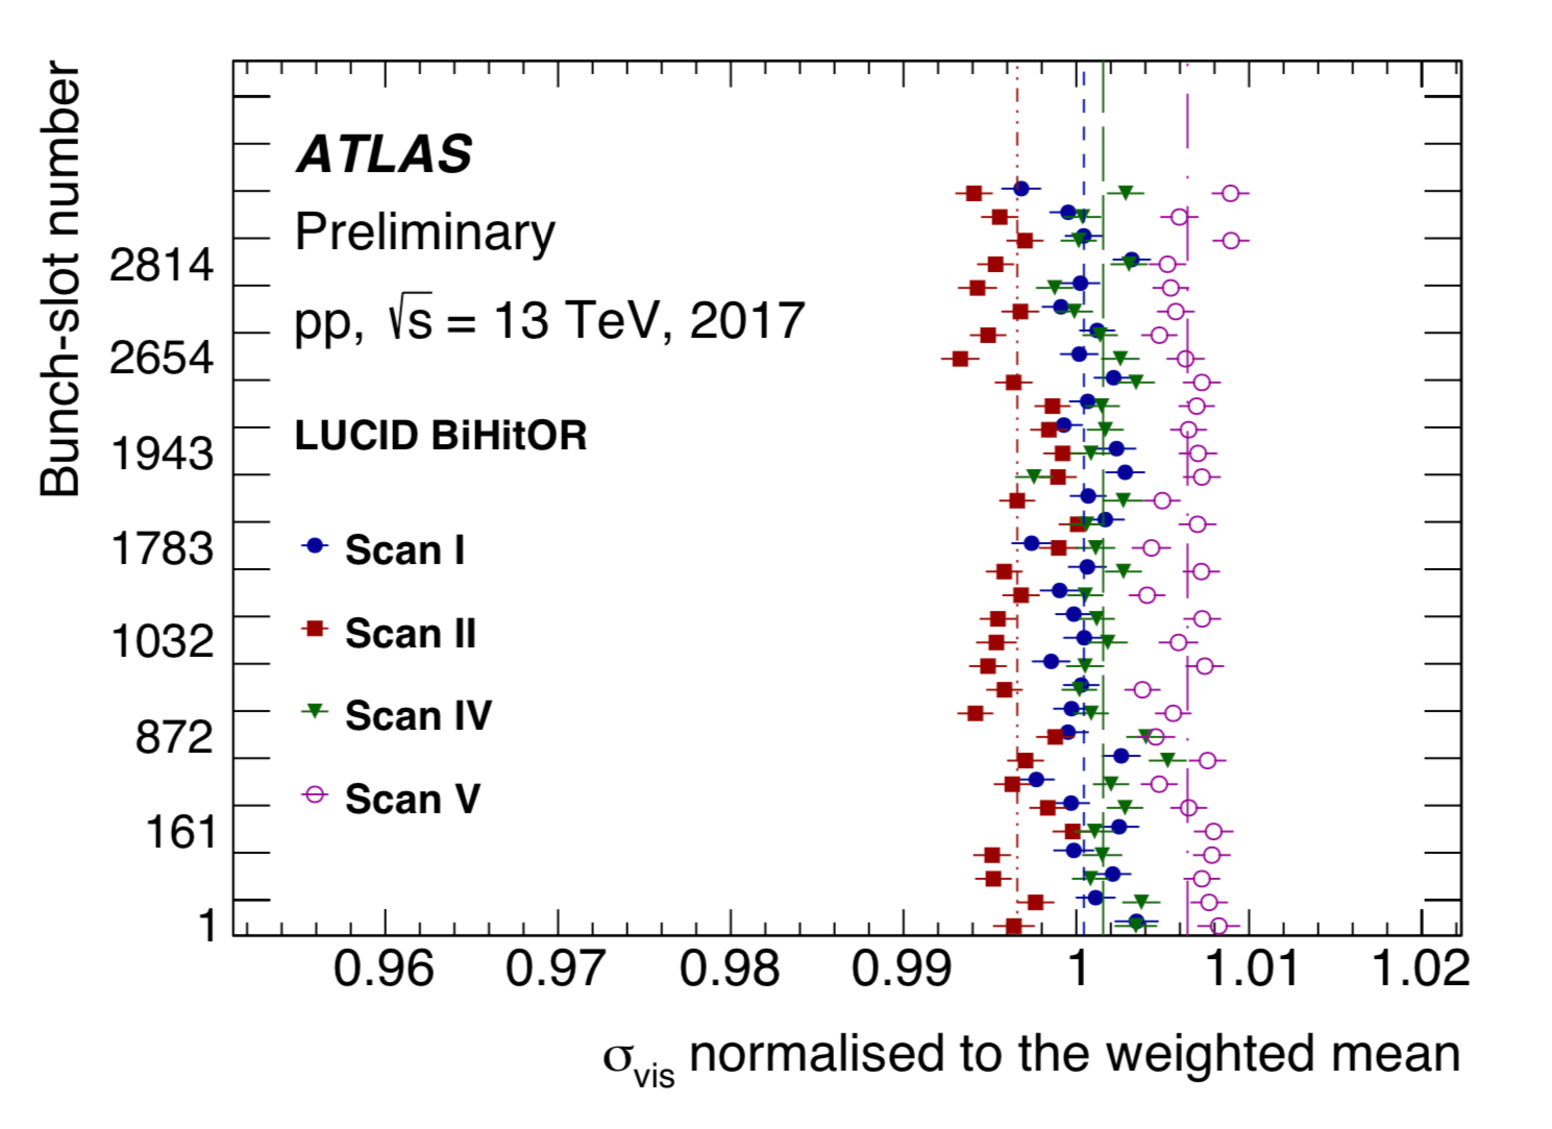
\includegraphics[width=0.43\textwidth]{figures/pmt_response/scan_to_scan.pdf}\label{fig:app:scantoscan}}
\subfigure{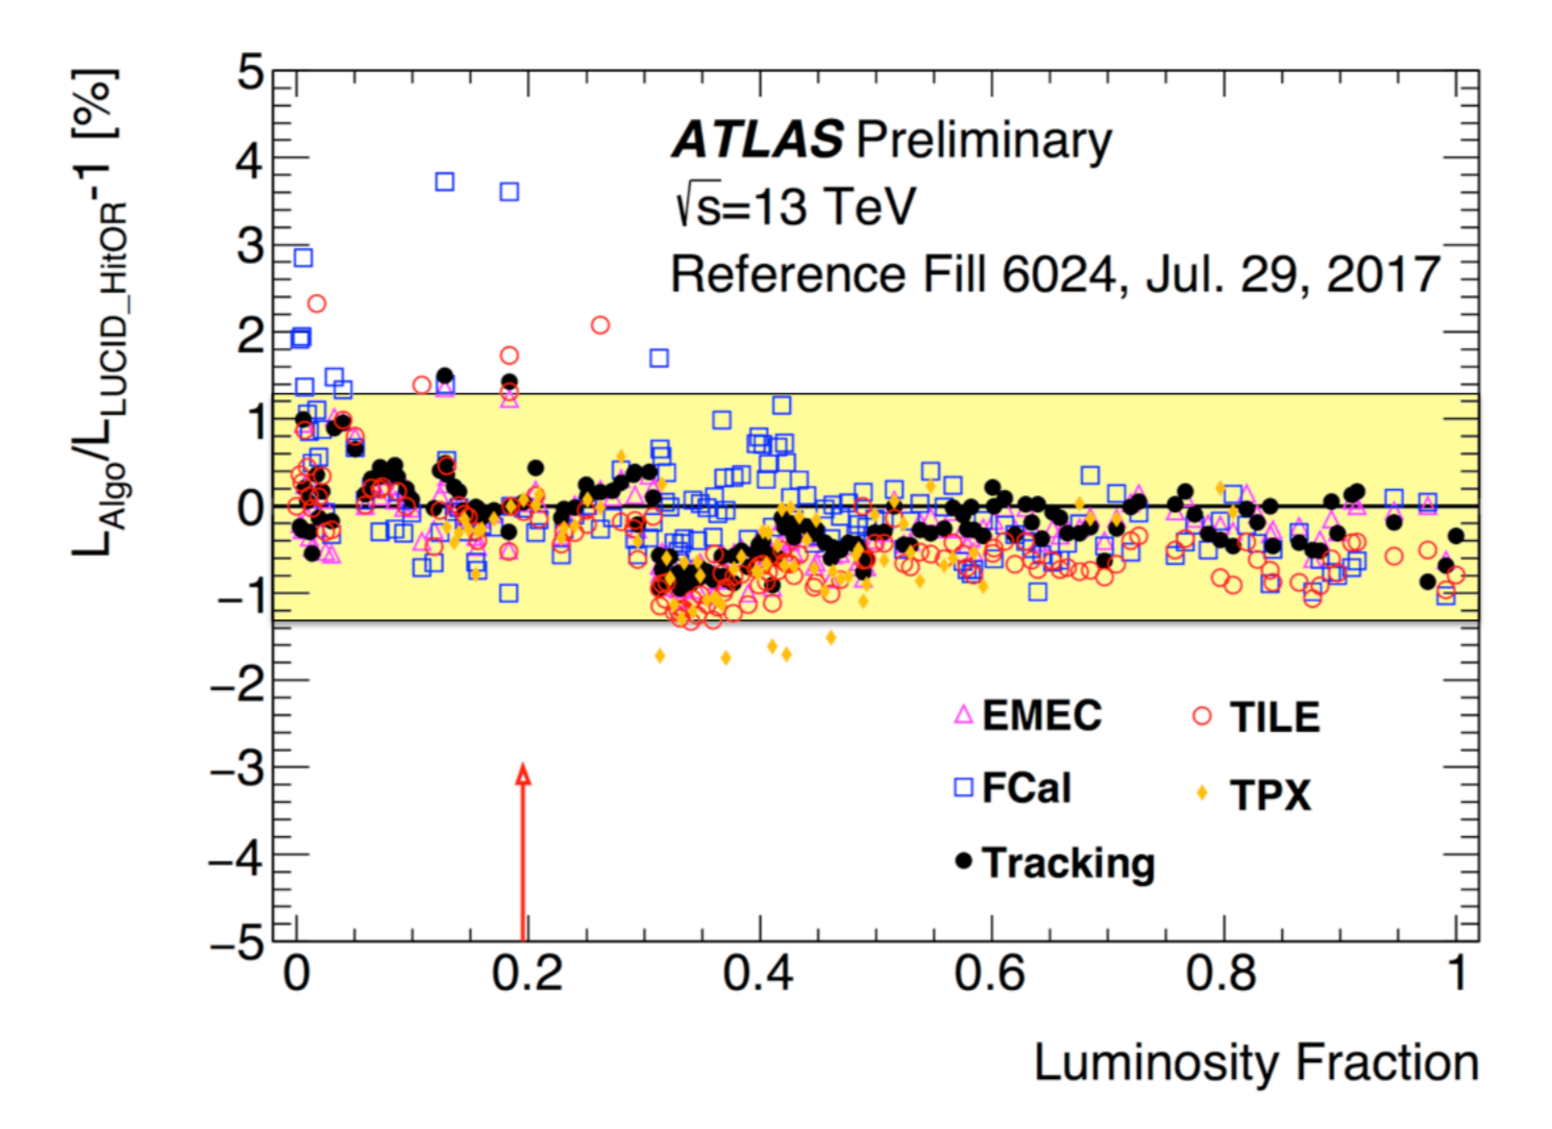
\includegraphics[width=0.55\textwidth]{figures/pmt_response/long_term_stability.pdf}\label{fig:app:longterm}}
\caption{\subref{fig:app:scantoscan} Scan-to-scan reproducibility. \subref{fig:app:longterm} Long-term stability.}
\label{fig:apppmt:othersyst}
\end{figure}


\section{Conclusion}

The calibration transfer uncertainty is one of the major sources of uncertainty in the \gls{atlas} luminosity 
measurement, and it has a relevant impact for analyses that rely on a precise luminosity measurement. 
The effect a non-linearity in the \gls{pmt} response with the increase in luminosity in the calibration transfer uncertainty from 
\gls{tilecal} has been studied. 
A correction has been derived that allows to reduce the calibration transfer uncertainty by 1 \% absolute.
This correction has been applied to the computation of the luminosity uncertainty released in March 2018, 
leading to a calibration transfer uncertainty of 1.3\%. 
This is summed in quadrature with the other uncertainty sources and 
the total luminosity uncertainty for the 2017 data-taking periods is estimated to be 2.4\%. 




